% Chapter Template

\chapter{The Application of New Genetic Algorithm Model in the Design of
Composite Material} % Main chapter title

\label{Chapter3} % Change X to a consecutive number; for referencing this chapter elsewhere, use \ref{ChapterX}

\section{Case1: Design of cross-ply Laminate}
%\section{Introduction}
Composite materials offer improved strength, stiffness, fatigue, corrosion resistance, etc., over
conventional materials, and are widely used as materials for applications ranging from the automotive to shipbuilding
industry, electronic packaging to golf clubs, and medical equipment to homebuilding. However, the high
cost of fabrication of composites is a critical drawback to its application. For example, the
graphite/epoxy composite part may cost as much as $650$ to $900$ per kilogram. In contrast, the price
of glass/epoxy is about 2.5 times less. Manufacturing techniques such as sheet molding compounds and
structural reinforcement injection molding are used to lower the costs for manufacturing automobile parts.
An alternative approach is using hybrid composite materials.


The mechanical performance of a laminate composite is affected by a wide range of factors such as the
thickness, material, and orientation of each lamina. Because of manufacturing limitations, all these
variables are usually limited to a small set of discrete values. For example, the ply thickness is fixed,
and ply orientation angles are limited to a set of angles such as 0, 45, and 90 degrees in practice. So
the search process for the optimal design is a discrete optimization problem that can be solved by the
GA. To tailor a laminate composite, the GA has been successfully applied to solve laminate design
problems\cite{riche1993optimization,nagendra1996improved,sadagopan1998application,todoroki1998stacking,liu2000permutation,sivakumar1998optimum,walker2003technique,lin2004stacking,kang2005minimum,murugan2007target,akbulut2008optimum}.
The GA simulates the process of natural evolution, including selection, crossover, and mutation
according to Darwin's principle of ''survival of the fittest''. The known advantages of GAs are the
following: (i): GAs are not easily trapped in local optima and can obtain the global
optimum. (ii): GAs do not need gradient information and can be applied to discrete optimization
problems. (iii): GAs can not only find the optimal value in the domain but also maintain a
set of optimal solutions. However, the GA also has some disadvantages, for example, the GA
needs to evaluate the target functions many times to achieve the optimization, and the cost of the
search process is high. The GA consists of some basic parts, the coding of the design variable,
the selection strategy, the crossover operator, the mutation operator, and how to deal with constraints. For the
variable design part, there are two methods to deal with the representation of design variables, namely,
binary string and real value representation\cite{riche1993optimization,todoroki1998stacking}.
Michalewicz\cite{zbigniew1996genetic} claimed that the performance of floating-point representation was
better than binary representation in the numerical optimization problem. Selection strategy plays a
critical role in the GA, which determines the convergence speed and the diversity of the population. To
improve search ability and reduce search costs, various selection methods have been invented, and they
can be divided into four classes: proportionate reproduction, ranking, tournament, and
genitor(or ''steady state'') selection. In the optimization of laminate composite design, the roulette
wheel\cite{riche1993optimization,seresta2007optimal}, where the possibility of an individual to be
chosen for the next generation is proportional to the fitness.
Soremekun et al.\cite{soremekun2001composite} showed that the generalized elitist strategy outperformed a
single individual elitism in some special cases.

Data structure, repair strategies, and penalty functions\cite{le1995improved} are the most commonly used
approaches to resolve constrained problems in the optimization of composite structures. Symmetric
laminates are widely used in practical scenarios, and data structures can be used to fulfill symmetry
constraints, which consists of coding half of the laminate and considering the rest with the
opposite orientation. Todoroki\cite{todoroki1998stacking} introduced a repair strategy that can scan the chromosome and
repair the gene on the chromosome if it does not satisfy the contiguity constraint. The comparison of
repair strategies in a permutation GA with the same orientation was presented by Liu et al.\cite{liu2000permutation}, and it
showed that the Baldwinian repair strategy can substantially reduce the cost of constrained optimization.
Haftka and Todoroki\cite{riche1993optimization} used the GA to solve the laminate stacking sequence problem using a penalty function subject to
buckling and strength constraints.

In typical engineering applications, composite materials are under very complicated loading
conditions, not only in-plane loading but also out-of-plane loading. Most of the studies on the
optimization of the laminate composite material minimized the
thickness\cite{abu1998optimum,walker2003technique},
weight\cite{fang1993design,deka2005multiobjective,park2008improved}, and cost and
weight\cite{deka2005multiobjective,omkar2008artificial}, or maximized the static strength of
the composite laminates for a targeted
thickness\cite{walker2003technique,lin2004stacking,kim2007development,gholami2020multi}. 
In the present study,
the cost and weight of laminates are minimized by modifying the objective function.

To check the feasibility of a laminate composite by imposing a strength constraint, failure
analysis of a laminate is performed by applying suitable failure criteria. The failure criteria of
laminated composites can be classified into three classes: non-interactive theories (e.g., maximum
strain), interactive theories (e.g., Tsai-wu), and partially interactive theories (e.g., Puck failure
criterion). Previous researchers adopted the first-ply-failure approach using Tsai-wu
failure
theory\cite{massard1984computer,reddy1987first,fang1993design,soeiro1994multilevel,pelletier2006multi,jadhav2007parametric,omkar2008artificial,choudhury2019failure},
Tsai-Hill\cite{martin1987optimum,soares1995discrete}, the maximum stress\cite{watkins1987multicriteria}, or the maximum strain\cite{watkins1987multicriteria}
static failure criteria. Akbulut\cite{akbulut2008optimum} used the GA to minimize the thickness of composite laminates with
Tsai-Hill and maximum stress failure criteria, and the advantage of this method is it avoids spurious
optima. Naik et al.\cite{naik2008design}
minimized the weight of laminated composites under restrictions with a
failure mechanism-based criterion based on the maximum strain and Tsai-wu. In the present study, Tsai-wu
Static failure criteria are used to investigate the feasibility of a laminate composite.

\section{Stress and Strain in a Laminate}
\begin{figure*}[!tb]
	\centering
	\includegraphics[width=\linewidth]{\ROOT/fig/lamina_local_global_axes.png}
	\caption{Local and global axes of an angle lamina.}
  	\label{fig:lamina}
\end{figure*}

\begin{figure}[!b]
	\centering
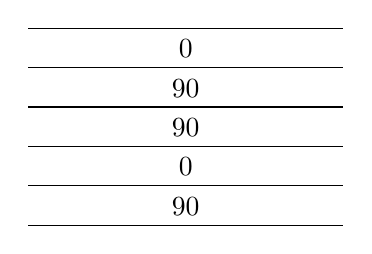
\begin{tikzpicture}
	\draw (0,0) -- (4,0);
	\draw (0,-0.5) -- (4,-0.5) node[midway, above] {$0$};
	\draw (0,-1) -- (4,-1) node[midway, above] {$90$} ;
	\draw (0,-1.5) -- (4,-1.5) node[midway, above] {$90$};
	\draw (0,-2) -- (4,-2) node[midway, above] {$0$};
	\draw (0,-2.5) -- (4,-2.5) node[midway, above] {$90$};
\end{tikzpicture}
\caption{Model for cross-ply laminate.}
\label{fig:cross_ply}
\end{figure}

A laminate structure consists of multiple lamina bonded together through their
thickness.  Considering a laminate composite plate that is subject to in-plane
loading of extension, shear, bending and torsion, the classical lamination
theory (CLT) is taken to calculate the stress and strain in the local and
global axes of each ply, as shown in Fig. \ref{fig:lamina}. Based on fiber
orientation, material, and fiber thickness, there are a few special cases of
laminate: the set of fiber angles in Fig. \ref{fig:cross_ply} only includes 0
and 90, which is called cross-ply laminate.
\begin{table*}[!ht]
\caption{Comparison of the graphite/epoxy and glass/epoxy properties.}
\centering
\begin{adjustbox}{width=1\textwidth}
\label{tab:mat}
\begin{tabular}{lcccc}
\toprule
Property								   & Symbol				  & Unit  &  Graphite/Epoxy  &  Glass/Epoxy   \\
\midrule
Longitudinal elastic modulus			   & $E_1$				  & GPa   &  181             &  38.6           \\
Traverse elastic modulus				   & $E_2$				  & GPa   &  10.3            &  8.27           \\
Major Poisson's ratio					   & $v_{12}$			  &       &  0.28            &  0.26           \\
Shear modulus							   & $G_{12}$			  & GPa   &  7.17            &  4.14           \\
Ultimate longitudinal tensile strength     & $(\sigma_1^T)_{ult}$ & MP    &  1500            &  1062            \\
Ultimate longitudinal compressive strength & $(\sigma_1^C)_{ult}$ & MP    &  1500            &  610             \\
Ultimate transverse tensile strength       & $(\sigma_2^T)_{ult}$ & MPa   &  40              &  31              \\
Ultimate transverse compressive strength   & $(\sigma_2^C)_{ult}$ & MPa   &  246             &  118              \\
Ultimate in-plane shear strength           & $(\tau_{12})_{ult}$  & MPa   &  68              &  72               \\
Density                                    & $\rho$               & $g/cm^3$  &  1.590           &  1.903               \\
Cost                                       &                      &           &  2.5             &  1               \\
\bottomrule
\end{tabular}
\end{adjustbox}
\end{table*}



\subsection{Stress and Strain in a Lamina}
For a single lamina, the stress-strain relation in local axis 1-2 is:
\begin{equation}
    \begin{bmatrix}
        \sigma _1\\
        \sigma _2\\
        \tau_{12}
    \end{bmatrix}
    =
    \begin{bmatrix}
        Q_{11} & Q_{12} & 0\\
        Q_{12} & Q_{22} & 0\\
        0      &  0     & Q_{66}
    \end{bmatrix}
    \begin{bmatrix}
        \varepsilon_1\\
        \varepsilon_2\\\gamma_{12}
	\end{bmatrix} \textstyle{,}
\end{equation}
where $Q_{ij} $ are the stiffnesses of the lamina that are related

to engineering elastic constants given by
\begin{equation}
    \begin{split}
    &Q_{11}=\frac{E_1}{1-v_{12}v_{21}}\textstyle{,}\\
    &Q_{22}=\frac{E_2}{1-v_{12}v_{21}}\textstyle{,}\\
    &Q_{66}=G_{12}\textstyle{,}\\
    &Q_{12}=\frac{v_{21}E_2}{1-v_{12}v_{21}}\textstyle{,}\\
    \end{split}
\end{equation}

where $E_1, E_2, v_{12}, G_{12} $ are four independent engineering elastic constants, which are defined as follows: $E_1 $ is the longitudinal Young's modulus, $E_2 $ is the transverse Young's modulus, $v_{12} $ is the major Poisson's ratio, and $G_{12} $ is the in-plane shear modulus.

Stress strain relation in the global x-y axis:
\begin{equation}
	\left[\begin{array}{l}\sigma _{x} \\ 
		\sigma _{y} \\ 
		\tau_{xy}
	\end{array}\right]=
	\left[\begin{array}{lll}
		\bar{Q}_{11} & \bar{Q}_{12} & \bar{Q}_{16}\\ 
	    \bar{Q}_{12} & \bar{Q}_{22} & \bar{Q}_{26} \\ 
	    \bar{Q}_{16} & \bar{Q}_{26} &\bar{Q}_{66}
	\end{array}\right]\left[\begin{array}{l}\varepsilon_{x} \\ 
	\varepsilon_{y}\\ \gamma_{x y}\end{array}\right] \textstyle{,}
\end{equation}
where

\begin{equation}
	\begin{array}{l}
		\resizebox{.35\textwidth}{!}{$\bar{Q}_{11}=Q_{11} c^{4}+Q_{22} s^{4}+2\left(Q_{12}+2
		Q_{66}\right) s^{2} c^{2}$} \textstyle{,}\\
		\resizebox{.35\textwidth}{!}{$\bar{Q}_{12}=\left(Q_{11}+Q_{22}-4 Q_{66}\right) s^{2}
		c^{2}+Q_{12}\left(c^{4}+s^{2}\right)$} \textstyle{,}\\
		\resizebox{.35\textwidth}{!}{$\bar{Q}_{22}=Q_{11} s^{4}+Q_{22} c^{4}+2\left(Q_{12}+2
		Q_{66}\right) s^{2} c^{2}$} \textstyle{,}\\
		\resizebox{.4\textwidth}{!}{$\bar{Q}_{16}=\left(Q_{11}-Q_{12}-2 Q_{66}\right) c^{3} s-\left(Q_{22}-Q_{12}-2Q_{66}\right) s^{3} c$}\textstyle{,}
		 \\ 
		\resizebox{.4\textwidth}{!}{$\bar{Q}_{26}=\left(Q_{11}-Q_{12}-2 Q_{66}\right) c s^{3}-\left(Q_{22}-Q_{12}-2 Q_{66}\right)c^{3} s$}\textstyle{,}
		 \\ 
	\resizebox{.4\textwidth}{!}	{$\bar{Q}_{66}=\left(Q_{11}+Q_{22}-2 Q_{12}-2 Q_{66}\right)
	s^{2}c^{2}+Q_{66}\left(s^{4}+c^{4}\right)$}\textstyle{.}\\
	\end{array}
\end{equation}


The c and s denote $cos\theta $ and $sin\theta $, respectively.

The local and global stresses in an angle lamina are related

to each other through the angle of the lamina $\theta $
\begin{equation}\left[\begin{array}{l}\sigma _{1} \\ \sigma _{2} \\ \tau_{12}\end{array}\right]=[T]\left[\begin{array}{l}\sigma _{x} \\ \sigma _{y} \\\tau_{xy}\end{array}\right]
\end{equation}

where
\begin{equation}[T]=\left[\begin{array}{ccc}c^{2} & s^{2} & 2 s c \\ s^{2} & c^{2} & -2 s c \\ -s c & s c &c^{2}-s^{2}\end{array}\textstyle{.}\right] 
\end{equation}



\subsection{Stress and Strain in a Laminate}
\begin{equation} \label{eq:force_and_moments}
	\begin{array}{l}
		\begin{aligned}
	\begin{bmatrix}
		N_x \\
		N_y \\
		N_{xy}
	\end{bmatrix}
	&=
	\begin{bmatrix}
		A_{11} & A_{12} & A_{16} \\
		A_{12} & A_{22} & A_{26} \\
		A_{16} & A_{26} & A_{66} 
	\end{bmatrix}
    \begin{bmatrix}
		\varepsilon_x^0 \\
        \varepsilon_y^0 \\
		\gamma_{xy}^0
    \end{bmatrix}   \\
	&+               
	\begin{bmatrix}
		B_{11} & B_{12} & B_{16} \\
		B_{11} & B_{12} & B_{16} \\
		B_{16} & B_{26} & B_{66} 
	\end{bmatrix}
	\begin{bmatrix}
		k_x \\
		k_y \\
		k_{xy} 
	\end{bmatrix}  \\
\end{aligned} \\ \\
\begin{aligned}
	\begin{bmatrix}
		M_x \\
		M_y \\
		M_{xy}
	\end{bmatrix}
	&=
	\begin{bmatrix}
		B_{11} & B_{12} & B_{16} \\
		B_{12} & B_{22} & B_{26} \\
		B_{16} & B_{26} & B_{66} 
	\end{bmatrix}
    \begin{bmatrix}
		\varepsilon_x^0 \\
        \varepsilon_y^0 \\
		\gamma_{xy}^0
    \end{bmatrix} \\ 
	&+  
	\begin{bmatrix}
		D_{11} & D_{12} & D_{16} \\
		D_{11} & D_{12} & D_{16} \\
		D_{16} & D_{26} & D_{66} 
	\end{bmatrix}
	\begin{bmatrix}
		k_x \\
		k_y \\
		k_{xy} 
	\end{bmatrix}
\end{aligned}
	\end{array}
\end{equation}


$N_x,N_y $  - normal force per unit length

$N_{xy} $  - shear force per unit length

$M_x, M_y $ - bending moment per unit length

$M_{xy} $  - twisting moments per unit length

$\varepsilon^{0}, k $- mid-plane strains and curvature of a laminate in x-y coordinates

The mid-plane strain and curvature is given by
\begin{equation}
    \begin{split}
	&A_{ij}=\sum_{k=1}^{n}(\overline{Q_{ij}})_k(h_k-h_{k-1})  i=1,2,6, j=1,2,6 \textstyle{,}\\
	&B_{ij}=\frac{1}{2}\sum_{k=1}^{n}(\overline{Q_{ij}})_k(h^2_k - h_{k-1}^2)  i=1,2,6, j=1,2,6 \textstyle{,}\\
	&D_{ij}=\frac{1}{3}\sum_{k=1}^{n}(\overline{Q_{ij}})_k(h^3_k - h_{k-1}^3) i=1,2,6, j=1,2,6 \textstyle{,}\\
    \end{split}
\end{equation}

where the [A], [B], and [D] matrices are called the extensional, coupling, and bending stiffness matrices.

\section{Failure Theory}

\subsection{Failure Process}
A laminate will fail under increasing mechanical loading; however, the procedure of laminate failure may not
be catastrophic.
 In some cases, some layers fail first, and the rest are able to continue to take additional loading
 until all the plies fail. A ply is fully discounted when a ply fails; then, the ply is replaced
by a near-zero stiffness and strength. 
The procedure for finding the first ply failure in the present
study follows the fully discounted method:

\begin{enumerate}
\item Compute the reduced stiffness matrix [Q] referred to as the local axis for each ply using its four engineering elastic constants $E_1 $, $E_2 $, $E_{12} $, and $G_{12} $.

\item Calculate the transformed reduced stiffness $[\bar{Q}] $ referring to the global coordinate system (x, y) using the reduced stiffness matrix [Q] obtained in step 1 and the ply angle for each layer.

\item  Given the thickness and location of each layer, the three laminate stiffness matrices [A], [B], and [D] are determined.

\item  Apply the forces and moments, $[N]_{xy}, [M]_{xy} $ solve
Equation \ref{eq:force_and_moments}, and calculate the middle plane strain $[\sigma ^{0}]_{xy} $ and curvature $[k]_{xy} $.

\item Determine the local strain and stress of each layer under the applied load.

\item  Use the ply-by-ply stress-strain and related failure theories to determine the strength ratio.
\end{enumerate}

\subsection{Tsai-wu Failure Theory}

Many different theories about the failure of an angle lamina have been developed for a
unidirectional lamina, such as the maximum stress failure theory, maximum strain failure theory,
Tsai-Hill failure theory, and Tsai-Wu failure theory. The failure theories of a lamina are based on
the stresses in the local axes in the material. There are four normal strength parameters and one shear
stress for a unidirectional lamina. The five strength parameters are:

$(\sigma _1^{T})_{ult}= $ ultimate longitudinal tensile strength

$(\sigma _1^{C})_{ult}= $ ultimate longitudinal compressive strength

$(\sigma _2^{T})_{ult}= $ ultimate transverse tensile strength

$(\sigma _2^{C})_{ult}= $ ultimate transverse compressive strength 

$(\tau_{12})_{ult}= $ and ultimate in-plane shear strength

In the present study, Tsai-wu failure theory is taken to decide whether a lamina fails,
because this theory is more general than the Tsai-Hill failure theory, which considers two
different situations, the compression and tensile strengths of a lamina. A lamina is considered to fail
if \begin{equation} \label{eq:tsai_wu}
\begin{split}
	H_1 \sigma_1  & + H_2 \sigma_2 + H_6 \tau_{12} + H_{11}\sigma_1^2 + H_{22} \sigma_2^2 \\
				  & + H_{66}  \tau_{12}^2 + 2H_{12}\sigma_1\sigma_2 < 1
\end{split}
\end{equation}

is violated, where

\begin{equation} \label{eq:sr}S R=\frac{\text {Maximum Load}}{\text {Load Applied}}
\end{equation}

The maximum load refers to that can be applied using Tsai-wu failure theory.


\section{Optimum Design of a Laminate Composite}


\begin{figure}
\begin{center}
	\begin{tikzpicture}[thick, scale=0.6, every node/.style={transform shape}]
	\tikzstyle{rec} = [rectangle, minimum width=4cm, minimum height=0.8cm,
	text centered, draw=black]
	\tikzstyle{subgroup} = [rectangle, minimum width=1.5cm, minimum height=0.6cm,
	text centered, draw=black]
	\tikzstyle{bigsubgroup} = [rectangle, minimum width=2.5cm, minimum height=0.6cm,
	text centered, draw=black]
	% population
	\node (population) [rec] {population};
	% active group
	\node (active_group_1) at ($(population.south)+(-3cm, -2.0cm)$) [subgroup]
		{active group};
	\node (active_group_2) at ($(active_group_1.south)+(0cm, -2.0cm)$)
		[subgroup] {active parents};
	\draw[->] (population.south) -- (active_group_1.north);
	\draw[->] (active_group_1.south) -- (active_group_2.north);
	% potential group
	\node (potential_group_1) at ($(population.south)+(0cm, -2.0cm)$) [subgroup]
		{potential group};
	\node (potential_group_2) at ($(potential_group_1.south)+(0cm, -2.0cm)$)
		[subgroup] {potential parents};
	\draw[->] (population.south) -- (potential_group_1.north);
	\draw[->] (potential_group_1.south) -- (potential_group_2.north);
	\node at ($(potential_group_1.north)+(0cm, 1.0cm)$) {classification };
	\node at ($(potential_group_2.north)+(0cm, 1.0cm)$) {selection};
    % proper group
	\node (proper_group_1) at ($(population.south)+(3cm, -2.0cm)$) [subgroup]
		{proper group};
	\node (proper_group_2) at ($(proper_group_1.south)+(0cm, -2.0cm)$)[subgroup]
		{proper parents};
	\draw[->] (population.south) -- (proper_group_1.north);
	\draw[->] (proper_group_1.south) -- (proper_group_2.north);
	% crossover
	\node (after_cross_over) at ($(potential_group_2.south)+(0cm, -2.0cm)$) [rec] {};
	\node  at ($(after_cross_over.north)+(0cm, 1.0cm)$)  {crossover};
	\draw[-] ($(after_cross_over.south)+(-0.5cm,0cm)$) --
		($(after_cross_over.north)+(-0.5cm,0cm)$);
	\draw[->] (active_group_2.south) -- (after_cross_over.north);
	\draw[->] (potential_group_2.south) -- (after_cross_over.north);
	\draw[->] (proper_group_2.south) -- (after_cross_over.north);
	% mutation
	\node (active_group_3) at ($(after_cross_over.south)+(-2.2cm, -2.0cm)$)
		[subgroup] {active offspring};
	\node at ($(after_cross_over.south)+(0cm, -1.0cm)$) {mutation};
	\draw[->] ($(after_cross_over.south)+(-1cm,0cm)$)--(active_group_3.north);
	\node (poteni_and_prop) at ($(after_cross_over.south)+(2.2cm, -2.0cm)$)
		[bigsubgroup] {potential and proper offspring};
	\draw[->] ($(after_cross_over.south)+(1cm,0cm)$)--(poteni_and_prop.north);

	% final draw
	\draw[->] (poteni_and_prop.east) --($(poteni_and_prop.east) + (0.2cm,0cm)$) |- (population.east);
	\draw[->] (active_group_3.west) -- ($(active_group_3.west) + (-1cm,0cm)$)
		|- (population.west);
\end{tikzpicture}
\end{center}
\caption{GA Model\label{GA:model}}
\end{figure}

\subsection{Genetic Algorithm}
The GA starts off with multiple individuals with limited chromosome lengths, in which maybe none of
these individuals fulfill the safety factor constraint. The GA is assumed to derive appropriate
offspring based on the initial population as the GA continues. The classic way to handle the constrained
search of the GA is either to introduce repair strategies or use a penalty function. Here, a new
approach is developed to address the constrained GA search problem by modifying the selection
strategy.

Because of the existence of constraints, the population can be sorted by the
fitness (obtained by the objective function) but can also be sorted by the
constraint value obtained by the constraint function (assuming a constraint
function exists), so the parents of the next generation can be chosen by the
following three approaches. First, the population is sorted by fitness in an
ascending order, and individuals with smaller fitness are selected. These
selected individuals form a group named as proper group. Second, remove
individual which satisfies constraints, and sort population  by the difference
between the individual's constraint value and the threshold of the constraint
in a descending order, and individuals with bigger differences are chosen to be
the parents of next generation. The group which forms are called potential
group, and individual from this group is refered as  potential individual.
Third, the population is sorted by fitness from low to high after removing
individuals which fails to fit the constraints, select individuals with bigger
fitness, and these individuals form the proper group.  So the final parents
pool is consists of three groups, active group, potential group and proper
group.  The number of active individuals, potential individuals and proper
individuals are called, respectively, active number, potential numbers and
proper number. 

Figure \ref{fig:model} shows the flow chart of the proposed GA. First, the
population are divided into three groups, active group, potential group, and
proper group by fitness and constraint functions. Second, select appropriate
number of individuals from each group as parents, and the selection strategy
for every group doesn't need to be the same. 



At the beginning of the GA, no individual in the population is appropriate, which means the number
of proper individuals is nearly zero. Therefore, the GA can be divided into two stages according to whether
proper individuals are generated during the search process. During the initial stages, the number of
potential individuals gradually decreases from the maximum (which is the parent population) to the potential
number, while the number of proper individuals increases from zero to the proper number as the GA
continues. After the initial stage, both groups converge to the
potential number and proper number. To differentiate the current selection methods from
the following, the current GA is called the basic GA. In the following experiment, 50 percent of the
parents are potential individuals, and 50 percent of the parents are proper individuals.

The problem with this basic GA is premature and has weak local search ability; therefore, basic GAs are more likely
to get stuck in a local optimum. Therefore, to prevent the GA from experiencing early convergence and to improve the
local search performance, a new selection method is proposed, which ignores whether the
individuals satisfy the constraint or not and ranks individuals by their fitness. Individuals
selected by this method are called active individuals because they are assumed to always be in the
population. GAs with these active individuals are called improved GAs. In the improved GA, the parents
consist of three parts: active individuals, potential individuals, and proper individuals. In the
following experiment, 20 percent of the parent population are active individuals, 30 percent of the
parents are potential individuals, and the rest are proper individuals.

In the present study, the relevant parameters of the GA are shown in Table \ref{tab:ga}. The design
variables are the materials, number of layers, and ply orientation restricted to a discrete set of
angles ($0,\pm 45 \text{ and } 90 \text{ degrees} $). The possible materials are graphite/epoxy,
carbon/epoxy, and glass/epoxy and are represented by codes 0, 1 and 2, respectively.


\begin{table}[!ht]
\centering
\caption{GA parameters}
\begin{adjustbox}{width=0.45\textwidth}
\label{tab:ga}
\begin{tabular}{cc}
\toprule
Parameter				&  Value  \\
\midrule
Seed					& 1       \\
Population size			& 20      \\
Initial length range	& [3-15]  \\
Encoding				& Integer  \\
Crossover strategy		& One-point \\
Mutation strategy		& Mass mutation \\
\bottomrule
\end{tabular}
\end{adjustbox}
\end{table}

%\begin{figure*}[!htb]
%  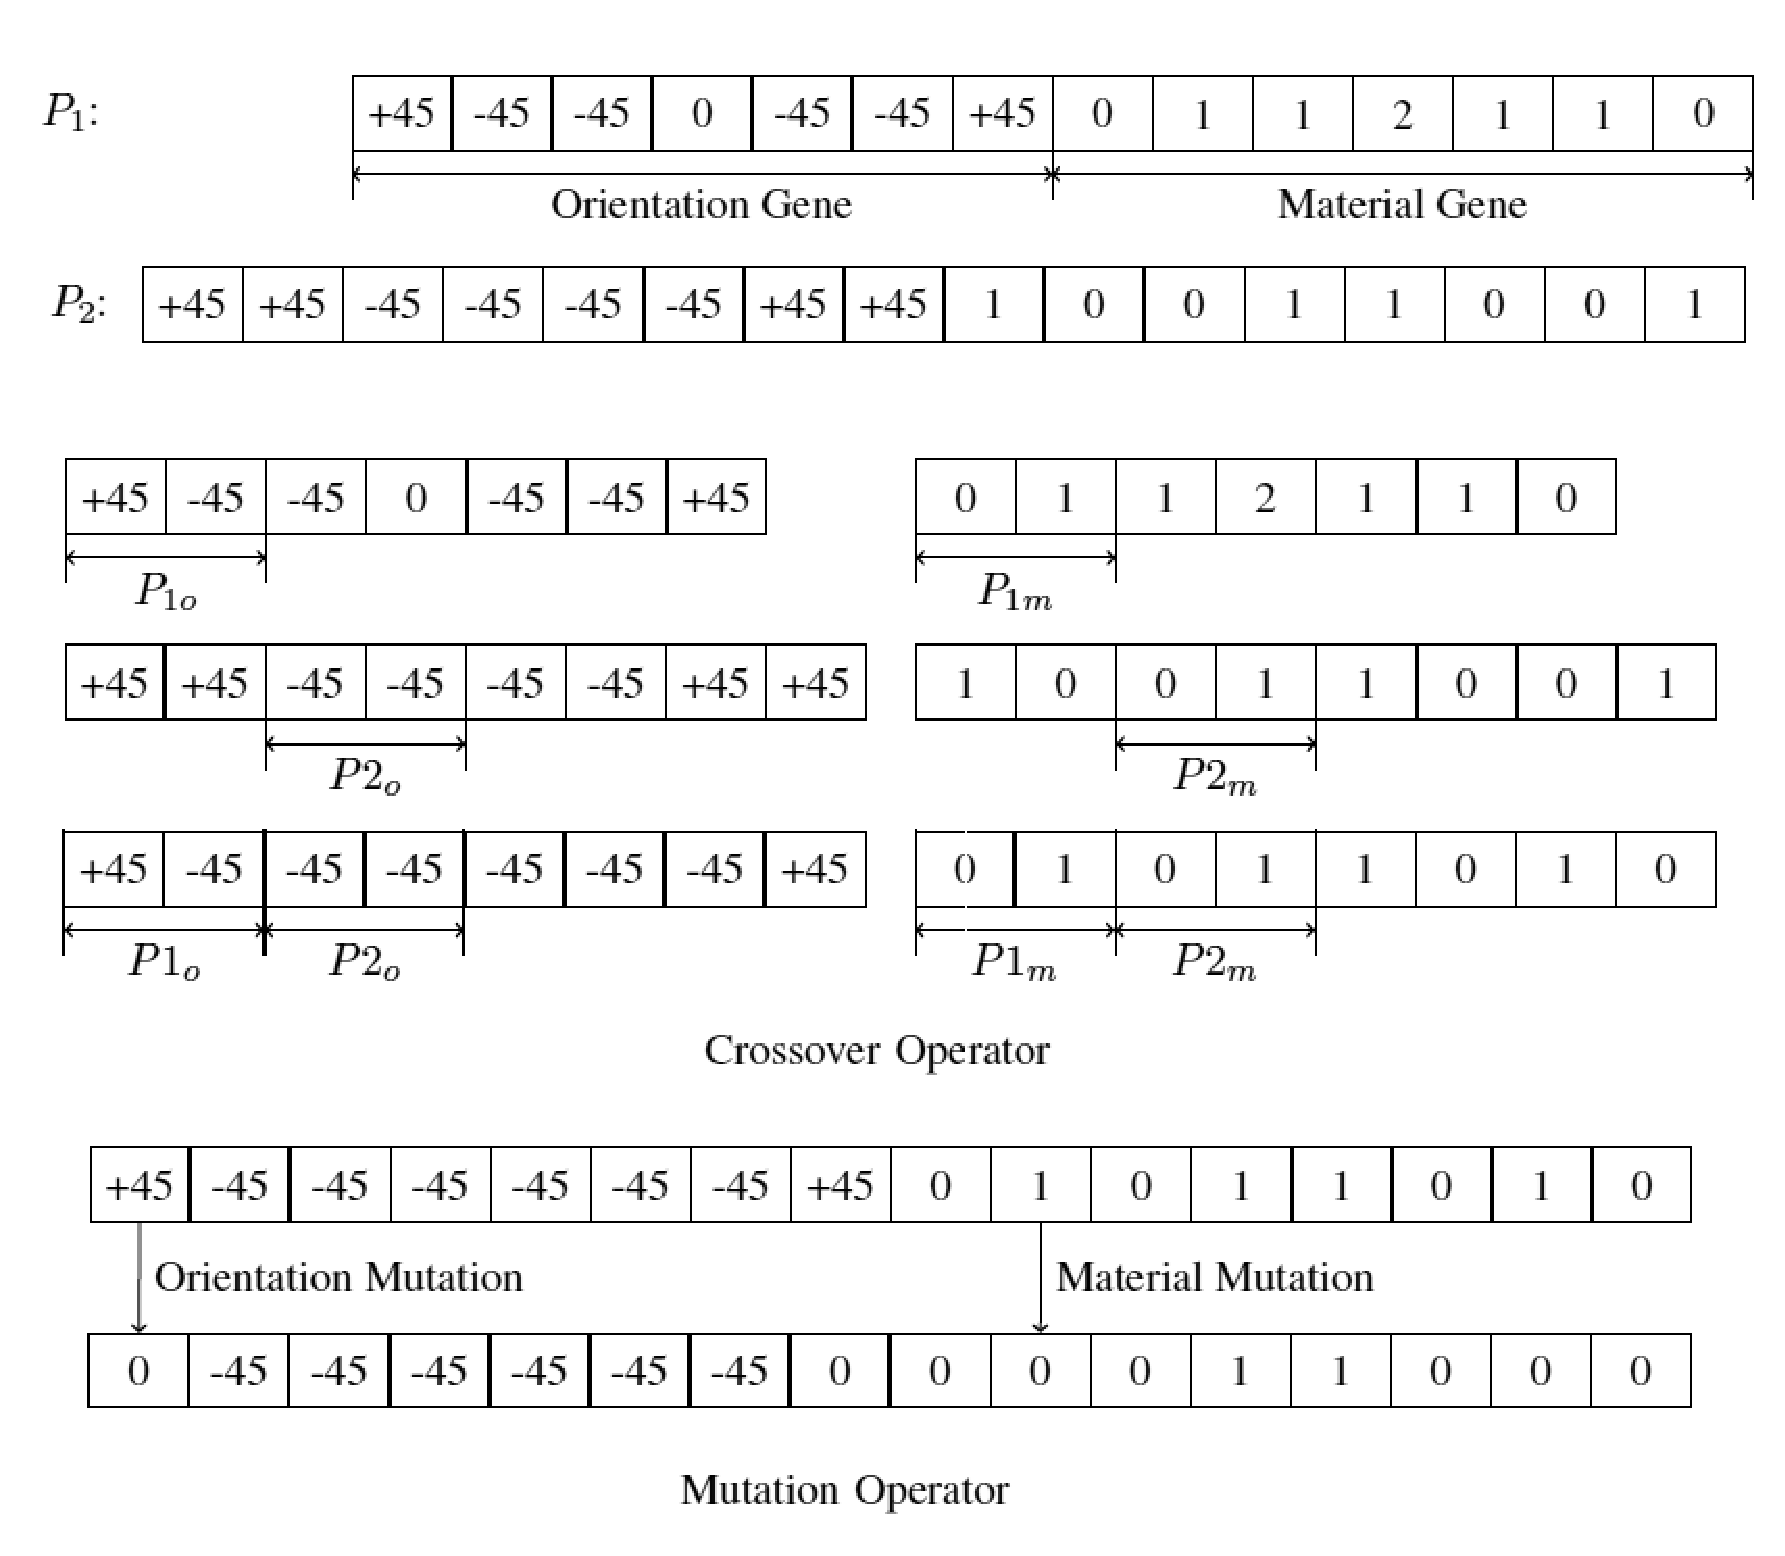
\includegraphics[width=\linewidth]{ga_operator}
%\caption{GA Operators\label{GA:operator}}
%\end{figure*}

The laminate chromosome is represented by a double-gene string that can be divided into two parts:
one part represents the angles, and the other part represents the materials (as shown in Figure
\ref{GA:operator}($P_1$)) . To maintain the diversity of the population, single-point crossover is
taken during the evolution process. The break points in the string are randomly chosen, and one of
the offspring of parent 1 (as shown in Figure \ref{GA:operator}($P_1$)) and parent 2 (as shown in
Figure \ref{GA:operator}($P_2$)) is obtained by combining the gene segments $P1_o$ and $P2_o$ and
$P1_m$ and $P2_m$, respectively. The gene code of the offspring laminate is
$[\text{+}45,\text{-}45,\text{-}45,\text{-}45,\text{-}45,\text{-}45,\text{-}45,0,1,0,1,1,0,1,0]$.


To prevent the search from becoming stuck in a local optimum, mutation is used to randomly change the
gene in the chromosome, and the offspring after the mutation operator is as shown in Figure
\ref{GA:operator}

The GA is a stochastic procedure that heavily depends on the generator of pseudorandom numbers. In
the present study, the standard Wichmann-Hill generator is used in the algorithm, which combines
three pure multiplicative congruent generators of moduli 30269, 30307 and 30323. The seed used
in this paper is 1.

\subsection{Design Problem I}

The aim is to minimize the mass of a laminate composite for a targeted strength
ratio based on the Tsai-wu failure theory. The design variable are the ply angles and the
number of layers.

Find: $\{\theta_k, n\}$ $\theta_k \in \{ 0,\text{+}45,\text{-}45,90\}$

Minimize: weight

Subject to: strength ratio and first ply failure constraint


\subsection{Design Problem II}
The aim is to minimize the weighted cost and weight of hybrid composite
laminates under various loading cases, so the design variable not only includes
the ply angles and number of layers but also the material of each lamina.


Find: $\{\theta_k,\text{mat}_k, n\}$ $\theta_k \in \{ 0,\text{+}45,\text{-}45,90\}$ $\text{mat}_k \in \{CA, GR, GL \}$

Minimize:
\begin{equation}
	F=\frac{\text { Cost }}{C_{\text {min }}}+\frac{\text { Weight }}{W_{\text {min }}}
\end{equation}

Subject to: strength ratio and first ply failure constraint


Here, CA, GF, and GL represent carbon/epoxy, graphite/epoxy, and glass/epoxy, and
$C_{\text{min}}$ and $W_{\text{min}}$ represent the cost and
weight corresponding to the laminates with a minimum cost and minimum weight
obtained from previous problem.

\section{Experiment}

\begin{figure}[!htb]
\setlength{\fboxsep}{0pt}%
\setlength{\fboxrule}{0pt}%
\begin{center}
\resizebox{.95\linewidth}{!}{
		\begin{tikzpicture}
		\tikzstyle{rec} = [rectangle, minimum width=0.8cm,minimum height=0.6cm, text
		centered, draw=black]
			\node (gene11) [rec] {90};
			\node (gene2) [rec] at ($(gene11.east)+(0.4cm,0)$)  {90};
			\node (gene3) [rec] at ($(gene2.east)+(0.4cm,0)$)  {0};
			\node (gene4) [rec] at ($(gene3.east)+(0.4cm,0)$)  {0};
			\node (gene5) [rec] at ($(gene4.east)+(0.4cm,0)$)  {0};
			\node (gene6) [rec] at ($(gene5.east)+(0.4cm,0)$)  {90};
			\node (gene7) [rec] at ($(gene6.east)+(0.4cm,0)$)  {90};
			\node (gene8) [rec] at ($(gene7.east)+(0.4cm,0)$)  {90};
			\node (gene9) [rec] at ($(gene8.east)+(0.4cm,0)$)  {90};
			\node (last) [rec] at ($(gene9.east)+(0.4cm,0)$)  {90};
			\node[text width=1cm] at ($(gene11.west)+(-0.3cm,0)$) {$P_1$:};
			\node (gene1) [rec] at ($(gene11.east)+(-0.4cm,-0.8cm)$) {0};
			\node (gene2) [rec] at ($(gene1.east)+(0.4cm,0)$)  {0};
			\node (gene3) [rec] at ($(gene2.east)+(0.4cm,0)$)  {90};
			\node (gene4) [rec] at ($(gene3.east)+(0.4cm,0)$)  {90};
			\node (gene5) [rec] at ($(gene4.east)+(0.4cm,0)$)  {90};
			\node (gene6) [rec] at ($(gene5.east)+(0.4cm,0)$)  {0};
			\node (gene7) [rec] at ($(gene6.east)+(0.4cm,0)$)  {0};
			\node (gene8) [rec] at ($(gene7.east)+(0.4cm,0)$)  {90};
			\node (gene9) [rec] at ($(gene8.east)+(0.4cm,0)$)  {0};
			\node (gene10) [rec] at ($(gene9.east)+(0.4cm,0)$)  {0};
			\node[text width=1cm] at ($(gene1.west)+(-0.3cm,0)$) {$P_2$:};
			\draw[-,white] ($(gene10.north)$)-- ++(0,-1.5cm);
			\node (label1) at ($(gene5.south)+(0cm,-0.5cm)$) {(a): Parents $P_1$ and $P_2$};
		\end{tikzpicture}
}

% offspring
\resizebox{.95\linewidth}{!}{
		\begin{tikzpicture}
			\tikzstyle{rec} = [rectangle, minimum width=0.8cm,minimum height=0.6cm, text
			centered, draw=black]
			\node (gene11) [rec] {90};
			\node (gene2) [rec] at ($(gene11.east)+(0.4cm,0)$) {90};
			\node (gene3) [rec] at ($(gene2.east)+(0.4cm,0)$)  {0};
			\node (gene4) [rec] at ($(gene3.east)+(0.4cm,0)$)  {0};
			\node (gene5) [rec] at ($(gene4.east)+(0.4cm,0)$)  {0};
			\node (gene6) [rec] at ($(gene5.east)+(0.4cm,0)$)  {0};
			\node (gene7) [rec] at ($(gene6.east)+(0.4cm,0)$)  {0};
			\node (gene8) [rec] at ($(gene7.east)+(0.4cm,0)$)  {90};
			\node (gene9) [rec] at ($(gene8.east)+(0.4cm,0)$)  {0};
			\node (last) [rec] at ($(gene9.east)+(0.4cm,0)$)  {0};
			\node[text width=1cm] at ($(gene11.west)+(-0.3cm,0)$) {$O_1$:};
			\node (gene1) [rec] at ($(gene11.east)+(-0.4cm,-0.8cm)$) {0};
			\node (gene2) [rec] at ($(gene1.east)+(0.4cm,0)$)  {0};
			\node (gene3) [rec] at ($(gene2.east)+(0.4cm,0)$)  {90};
			\node (gene4) [rec] at ($(gene3.east)+(0.4cm,0)$)  {90};
			\node (gene5) [rec] at ($(gene4.east)+(0.4cm,0)$)  {90};
			\node (gene6) [rec] at ($(gene5.east)+(0.4cm,0)$)  {90};
			\node (gene7) [rec] at ($(gene6.east)+(0.4cm,0)$)  {90};
			\node (gene8) [rec] at ($(gene7.east)+(0.4cm,0)$)  {90};
			\node (gene9) [rec] at ($(gene8.east)+(0.4cm,0)$)  {90};
			\node (gene10) [rec] at ($(gene9.east)+(0.4cm,0)$)  {90};
			\node[text width=1cm] at ($(gene1.west)+(-0.3cm,0)$) {$O_2$:};
			\draw[-,white] ($(gene10.north)$)-- ++(0,-1.5cm);
			\node (label1) at ($(gene5.south)+(0cm,-0.5cm)$) {(b): Offspring $O_1$ and $O_2$};
		\end{tikzpicture}
}

%mutation
\resizebox{.95\linewidth}{!}{
	\begin{tikzpicture}
	\tikzstyle{rec} = [rectangle, minimum width=0.8cm,minimum height=0.6cm, text
	centered, draw=black]
		\tikzstyle{rec} = [rectangle, minimum width=0.8cm,minimum height=0.6cm, text
		centered, draw=black]
		%\draw[help lines](-3,-3) grid (4,4);
		\node (gene11) [rec] {90};
		\node (gene2) [rec] at ($(gene11.east)+(0.4cm,0)$)  {90};
		\node (gene3) [rec] at ($(gene2.east)+(0.4cm,0)$)  {90};
		\node (gene4) [rec] at ($(gene3.east)+(0.4cm,0)$)  {$\cdots$};
		\node (gene5) [rec] at ($(gene4.east)+(0.4cm,0)$)  {90};
		\node (gene6) [rec] at ($(gene5.east)+(0.4cm,0)$)  {90};
		\node (gene7) [rec] at ($(gene6.east)+(0.4cm,0)$)  {0};
		\node (gene8) [rec] at ($(gene7.east)+(0.4cm,0)$)  {$\cdots$};
		\node (gene9) [rec] at ($(gene8.east)+(0.4cm,0)$)  {0};
		\node (last) [rec] at ($(gene9.east)+(0.4cm,0)$)  {0};
		\draw[<->,thick] (gene11.south) .. controls +(1.8,-0.4) .. (gene6.south)
			node[pos=0.5] {10} ;
		\draw[<->,thick] (gene7.south) .. controls +(1.3,-0.4) .. (last.south)
			node[pos=0.5] {9};
		\node[text width=1cm] at ($(gene11.west)+(-0.3cm,0)$) {$O_1$:};

		\node (label1) at ($(gene5.south)+(0cm,-0.8cm)$) {(c): Offspring $O_1$ after
			lenght mutation};

		\node (gene1) [rec] at ($(gene11.east)+(-0.4cm,-1.8cm)$) {90};
		\node (gene2) [rec] at ($(gene1.east)+(0.4cm,0)$)  {90};
		\node (gene3) [rec] at ($(gene2.east)+(0.4cm,0)$)  {90};
		\node (gene4) [rec] at ($(gene3.east)+(0.4cm,0)$)  {$\cdots$};
		\node (gene5) [rec] at ($(gene4.east)+(0.4cm,0)$)  {90};
		\node (gene6) [rec] at ($(gene5.east)+(0.4cm,0)$)  {0};
		\node (gene7) [rec] at ($(gene6.east)+(0.4cm,0)$)  {0};
		\node (gene8) [rec] at ($(gene7.east)+(0.4cm,0)$)  {$\cdots$};
		\node (gene9) [rec] at ($(gene8.east)+(0.4cm,0)$)  {0};
		\node (last) [rec] at ($(gene9.east)+(0.4cm,0)$)  {0};
		\node[text width=1cm] at ($(gene11.west)+(-0.3cm,0)$) {$O_1$:};
		\draw[-,white] ($(gene10.north)$)-- ++(0,-1.5cm);
		\node (label1) at ($(gene5.south)+(0cm,-0.5cm)$) {(d): Offspring $O_1$ 
			 after angle mutation};
	\end{tikzpicture}
}
\end{center}
\caption{Examples of crossover, length mutation, angle  mutation operator for proposed GA.}
\label{GA:operator}
\end{figure}


In the present study, the relevant parameters of the GA are shown in Table \ref{tab:ga}. The design
variables are the materials, number of layers, and ply orientation restricted to a discrete set of
angles ($0,\pm 45 \text{ and } 90 \text{ degrees} $). The possible materials are graphite/epoxy,
carbon/epoxy, and glass/epoxy and are represented by codes 0, 1 and 2, respectively.

Figure \ref{GA:operator} (b) shows 


\begin{table}[!htb]
\centering
\caption{Parameters of proposed GA model.}
\begin{adjustbox}{width=0.45\textwidth}
\label{tab:ga}
\begin{tabular}{lc}
\toprule
Parameter								&  Value  \\
\midrule
Population                              & 40        \\
Initial length range					& [3-15]    \\
Encoding								& Integer   \\
Percentage of parent                    & 0.5   \\
Percentage of active group				& 0.3   \\
Percentage of potential group			& 0.3   \\
Percentage of proper group				& 0.4   \\
Selection strategy for  active group	& Ranking   \\
Selection strategy for potential group	& Ranking   \\
Selection strategy for proper group	    & Ranking   \\
Crossover strategy			    		& One-point \\
Mutation strategy			    		& Mass mutation \\
Length mutation coefficient             & 5 \\
Angle mutation rate                     & 0.1 \\
\bottomrule
\end{tabular}
\end{adjustbox}
\end{table}


%\begin{figure*}[!htb]
%  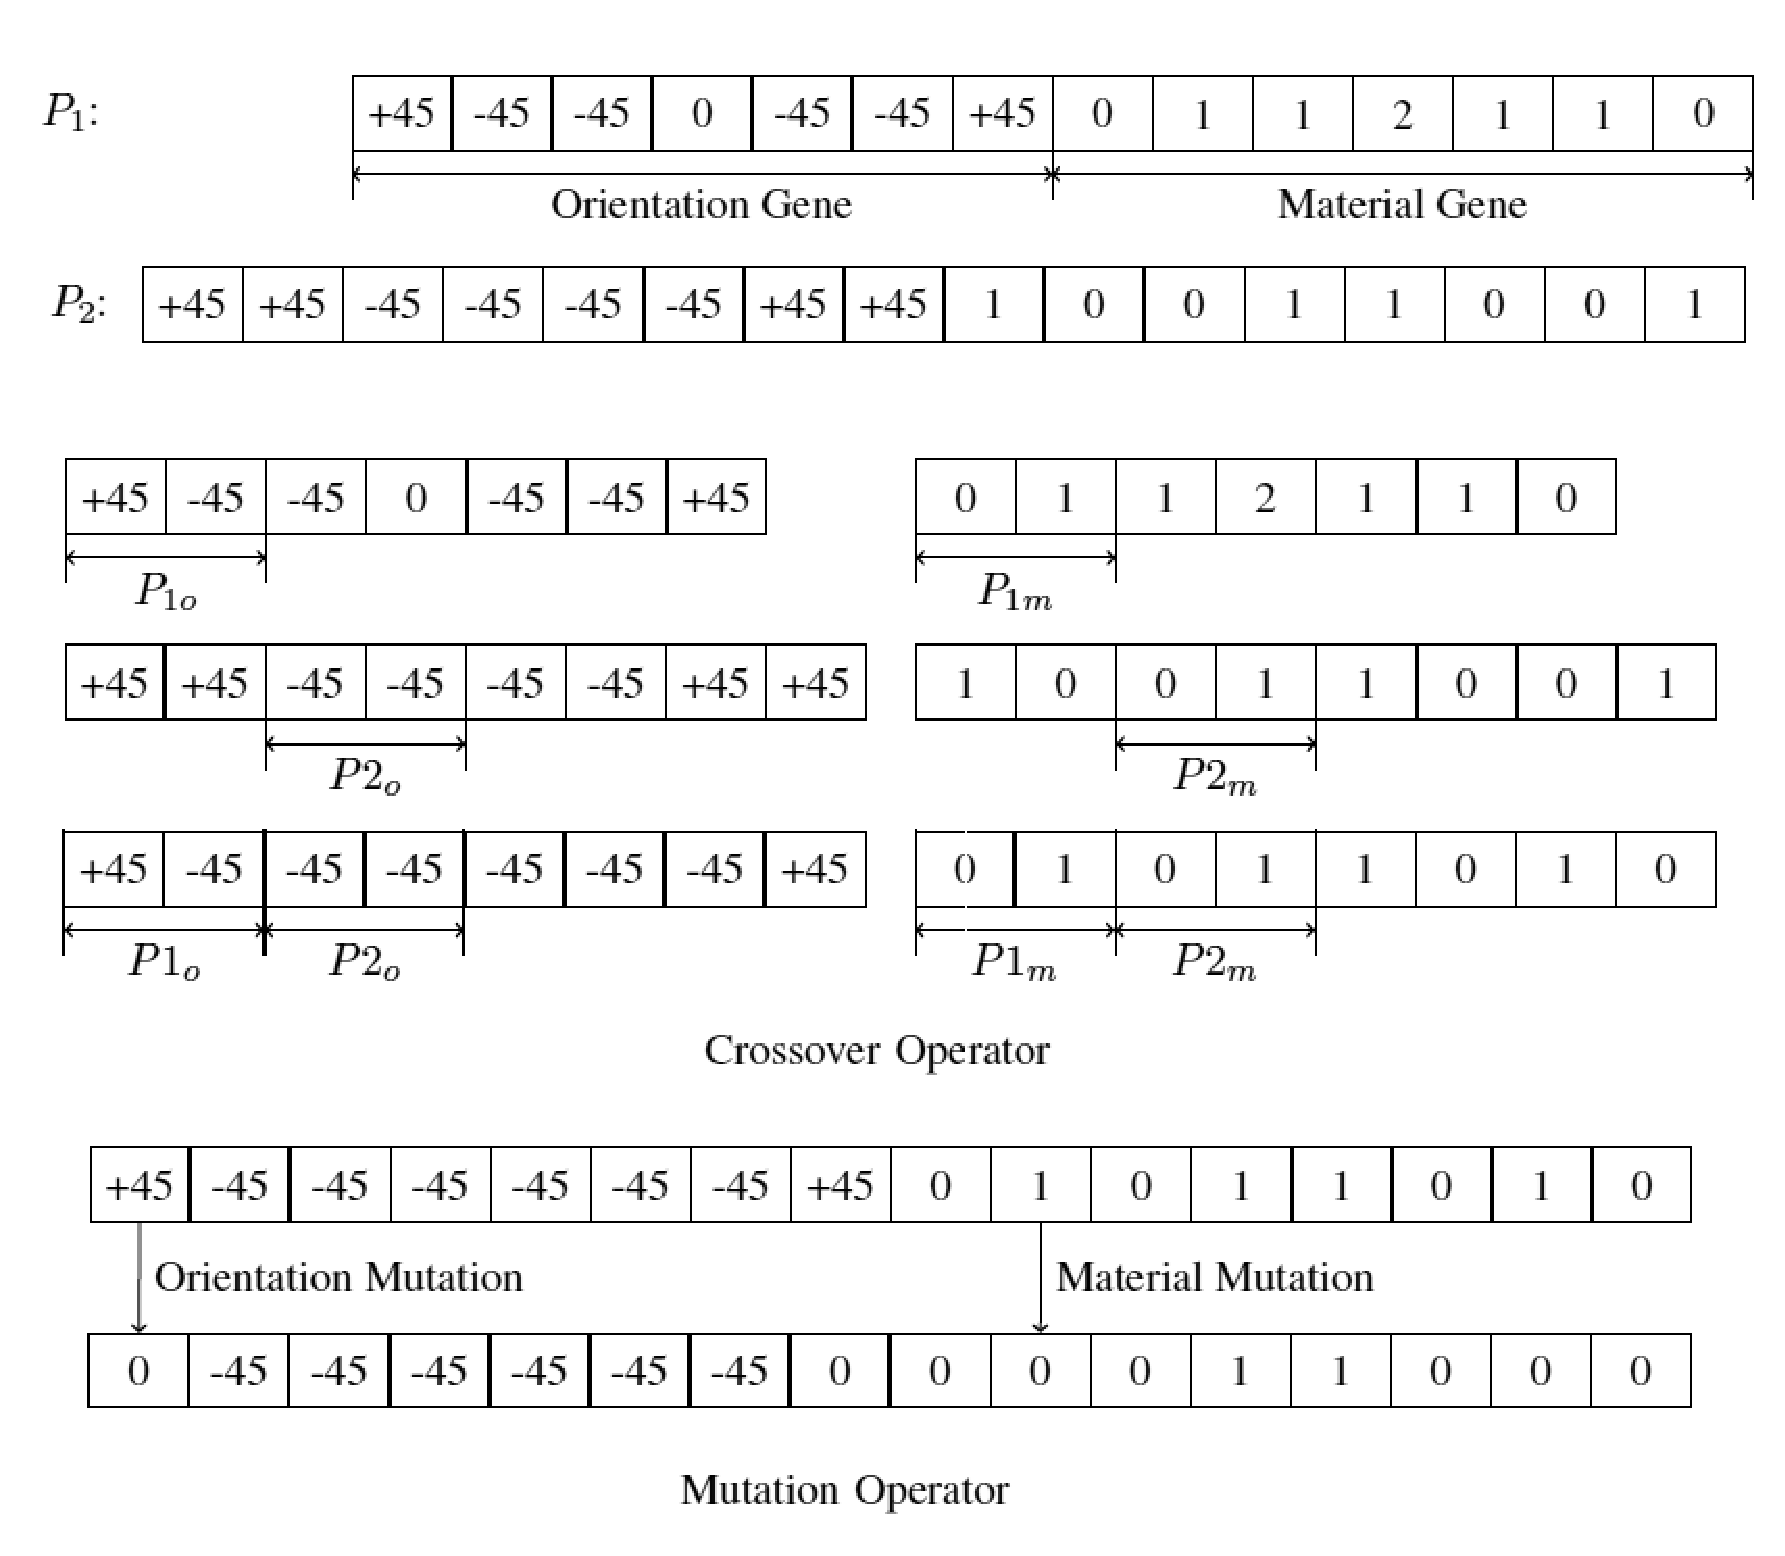
\includegraphics[width=\linewidth]{ga_operator}
%\caption{GA Operators\label{GA:operator}}
%\end{figure*}

The laminate chromosome is represented by a double-gene string that can be divided into two parts:
one part represents the angles, and the other part represents the materials (as shown in Figure
\ref{GA:operator}($P_1$)) . To maintain the diversity of the population, single-point crossover is
taken during the evolution process. The break points in the string are randomly chosen, and one of
the offspring of parent 1 (as shown in Figure \ref{GA:operator}($P_1$)) and parent 2 (as shown in
Figure \ref{GA:operator}($P_2$)) is obtained by combining the gene segments $P1_o$ and $P2_o$ and
$P1_m$ and $P2_m$, respectively. The gene code of the offspring laminate is
$[\text{+}45,\text{-}45,\text{-}45,\text{-}45,\text{-}45,\text{-}45,\text{-}45,0,1,0,1,1,0,1,0]$.


To prevent the search from becoming stuck in a local optimum, mutation is used to randomly change the
gene in the chromosome, and the offspring after the mutation operator is as shown in Figure
\ref{GA:operator}

The GA is a stochastic procedure that heavily depends on the generator of pseudorandom numbers. In
the present study, the standard Wichmann-Hill generator is used in the algorithm, which combines
three pure multiplicative congruent generators of moduli 30269, 30307 and 30323. The seed used
in this paper is 1.

\subsection{Design Problem I}

The aim is to minimize the mass of a laminate composite for a targeted strength
ratio based on the Tsai-wu failure theory. The design variable are the ply angles and the
number of layers.

Find: $\{\theta_k, n\}$ $\theta_k \in \{ 0,\text{+}45,\text{-}45,90\}$

Minimize: weight

Subject to: strength ratio and first ply failure constraint


\subsection{Design Problem II}
The aim is to minimize the weighted cost and weight of hybrid composite
laminates under various loading cases, so the design variable not only includes
the ply angles and number of layers but also the material of each lamina.


Find: $\{\theta_k,\text{mat}_k, n\}$ $\theta_k \in \{ 0,\text{+}45,\text{-}45,90\}$ $\text{mat}_k \in \{CA, GR, GL \}$

Minimize:
\begin{equation}
	F=\frac{\text { Cost }}{C_{\text {min }}}+\frac{\text { Weight }}{W_{\text {min }}}
\end{equation}

Subject to: strength ratio and first ply failure constraint


Here, CA, GF, and GL represent carbon/epoxy, graphite/epoxy, and glass/epoxy, and
$C_{\text{min}}$ and $W_{\text{min}}$ represent the cost and
weight corresponding to the laminates with a minimum cost and minimum weight
obtained from previous problem.
\section{Numerical Results and Discussion}


\begin{figure}[!htb]
	\centering
	\includegraphics[width=\linewidth]{fig/group_number.png}
\end{figure}

\begin{figure}[!htb]
	\centering
	\includegraphics[width=\linewidth]{fig/fitness_strength_ratio.png}
\end{figure}

A laminate composite with dimensions $1000 \times 1000 \times 0.165 mm^3$ for
each lamina is under various loading cases, and each CA, GF, and GL layer is
assumed to cost 8, 2.5 and 1 monetary units, respectively. The other
material properties are shown in Table \ref{tab:mat}. A carbon/epoxy ply is represented by "cr", a
graphite/epoxy ply by "gl", and a glass/epoxy ply by "gl".  In the present
experiment, the optimal composite system, layup, thickness, and number of
layers for a targeted strength ratio (2 in this paper) under two different
in-plane loading conditions is investigated.



\begin{table*}[!ht]
\caption{Comparison of the graphite/epoxy and glass/epoxy properties.}
\centering
\begin{adjustbox}{width=1\textwidth}
\label{tab:mat}
\begin{tabular}{lcccc}
\toprule
Property								   & Symbol				  & Unit  &  Graphite/Epoxy  &  Glass/Epoxy   \\
\midrule
Longitudinal elastic modulus			   & $E_1$				  & GPa   &  181             &  38.6           \\
Traverse elastic modulus				   & $E_2$				  & GPa   &  10.3            &  8.27           \\
Major Poisson's ratio					   & $v_{12}$			  &       &  0.28            &  0.26           \\
Shear modulus							   & $G_{12}$			  & GPa   &  7.17            &  4.14           \\
Ultimate longitudinal tensile strength     & $(\sigma_1^T)_{ult}$ & MP    &  1500            &  1062            \\
Ultimate longitudinal compressive strength & $(\sigma_1^C)_{ult}$ & MP    &  1500            &  610             \\
Ultimate transverse tensile strength       & $(\sigma_2^T)_{ult}$ & MPa   &  40              &  31              \\
Ultimate transverse compressive strength   & $(\sigma_2^C)_{ult}$ & MPa   &  246             &  118              \\
Ultimate in-plane shear strength           & $(\tau_{12})_{ult}$  & MPa   &  68              &  72               \\
Density                                    & $\rho$               & $g/cm^3$  &  1.590           &  1.903               \\
Cost                                       &                      &           &  2.5             &  1               \\
\bottomrule
\end{tabular}
\end{adjustbox}
\end{table*}

%\begin{figure*}[!htb]
%	\centering
%	\includegraphics[width=\linewidth]{lamina_local_global_axes.eps}
%\caption{Lamina}
% 	\label{fig:lamina}
%\end{figure*}



\begin{table*}[!htb]
\caption{The optimum lay-ups for the loading $N_x=1e6$ N}
\centering
\begin{adjustbox}{width=1\textwidth}
	\begin{tabular}{c|cc|cc}
		\toprule
		Cross Ply $[0_M/90_N]$         & \multicolumn{2}{c}{Previous Research} & \multicolumn{2}{c}{Current Research} \\
		\midrule																								  
		 Material       &  Glass-Epoxy & Graphite-Epoxy  & Glass-Epoxy & Graphite-Epoxy      \\ 
			  M         &  68          &    17           &  78		    &  18             \\
			  N         &  72          &    18           &  28		    &  8              \\
	no. of lamina(n)    &  140         &    35           &  106	    &  26                     \\
			 SR         &  2.01        &    2.10         &  2.03	    &  2.16            \\
		 weight         &  9.10        &    1.84         &  6.89	    &  102.5           \\
		\bottomrule
	\end{tabular}
\end{adjustbox}
\label{tab:comparsion}
\end{table*}


Table \ref{tab:comparsion} shows the optimal lay-up sequences by the variant GA
and  Choudhury and Mondal's\cite{choudhury2019failure} study. For the loading
case $Nx=1$ MPa m, the optimal lay-ups are a $[0_{68}/90_{72}]$  cross ply
laminate if glass-epoxy are taken, however,  in present study, a
$[0_{78}/90_{28}]$ glass-epoxy cross ply laminate has been found which
significantly reduces both the cost and weight with increasing laminate's SR;
If graphite-epoxy was used, compared with the $[0_{17}/90_{18}]$ cross ply
laminate, an alternative cross ply laminate is found, its lay-up is $[0_{18}/90_8]$.


The GA process can be divided into two phases by whether there are individuals that are appropriate
or not. During the initial phase, no individual's strength ratio is over the specified threshold, so
individuals with larger fitness are more likely to be chosen as parents, which is why the strength
ratio curves go all the way up to the specified threshold during the first stage. After the initial
phase, the GA produces many appropriate individuals, and then the target function is utilized, and
as shown in Fig. \ref{fig:NxNy}, the fitness curves tend to decrease, but the
strength ratio curves remain greater than the specified threshold.

\begin{table*}[!htb]
\caption{The optimum lay-ups for the loading $N_x=N_y=1e6$ N}
\centering
\begin{adjustbox}{width=1\textwidth}
	\begin{tabular}{cccccccc}
	\toprule
	coefficient		     &	 Material		               	 & case     & Stacking sequence   & Strength ratio  & Mass  &  Cost   & Layer    \\ 
	\midrule																															  
	\multirow{6}{*}{0.1} &	\multirow{3}{*}{glass-epoxy}   	 & worst     &                    &                 &        &         &       \\
						 &								     & best      &                    &                 &        &         &       \\
					     &									 & average   &                    &                 &        &         &    \\
						 &	\multirow{3}{*}{graphite-epoxy}	 & worst     &                    &                 &        &         &    \\
					     &								     & best      &               &                 &        &         &   \\
					     &								     & average   &               &                 &        &         &   \\
	\multirow{6}{*}{0.1} &	\multirow{3}{*}{glass-epoxy}   	 & worst     &                    &                 &        &         &       \\
						 &								     & best      &                    &                 &        &         &       \\
					     &									 & average   &                    &                 &        &         &    \\
						 &	\multirow{3}{*}{graphite-epoxy}	 & worst     &                    &                 &        &         &    \\
					     &								     & best      &               &                 &        &         &   \\
					     &								     & average   &               &                 &        &         &   \\
	\multirow{6}{*}{0.1} &	\multirow{3}{*}{glass-epoxy}   	 & worst     &                    &                 &        &         &       \\
						 &								     & best      &                    &                 &        &         &       \\
					     &									 & average   &                    &                 &        &         &    \\
						 &	\multirow{3}{*}{graphite-epoxy}	 & worst     &                    &                 &        &         &    \\
					     &								     & best      &               &                 &        &         &   \\
					     &								     & average   &               &                 &        &         &   \\
\end{tabular}
\end{adjustbox}
\label{tab:NxNy}
\end{table*}


In the first experiment, the applied stress is $N_x=N_y=1e6$ N. As shown in
Figure \ref{fig:NxNy}, Figures \ref{fig:NxNy}(a), (b), and (c) show the experimental results for a single material,
Figure \ref{fig:NxNy}(d) shows the results for the hybrid composite material.
 For the single materials, both the basic GA and improved
GA method obtained the optimal value, but the improved GA converged more slowly than the basic GA.
As seen from Table \ref{tab:NxNy}, a $[\text{-}45_{6}/\text{+}45_{6}]_s$ carbon/epoxy
laminate has the least weight, denoted by $W_{min}$, and a
$[\text{-}45_{35}/\text{+}45_{73}/\text{+}45_{35}]$ graphite/epoxy laminate has the lowest cost,
denoted by $C_{min}$. $W_{min}$ and $C_{min}$ were used to evaluate the fitness of the second
problem, which is the layup design of the hybrid composite material. As shown in subfigure d, the
improved GA obtained a more appropriate system layup, whose strength ratio was greater than the
specified safety factor, and the weight and cost are less than the result obtained by the basic GA method, as
shown in Table \ref{tab:NxNy}.
 Compared with the basic GA, the improved GA method showed more powerful
global search ability in the initial phase.


In the second case, the applied stress was $N_x=N_y=N_z=1e6$ N, and the experimental results were as
shown in the Figure \ref{fig:NxNyNz}. In the first experiment, as seen from Figure \ref{fig:NxNyNz}(a), the improved GA obtained a
better system layup than the result obtained by the basic GA. In the second experiment, as shown in Figure \ref{fig:NxNyNz}(b), during
the initial phase, the fitness curves of the basic GA and improved GA went all the way up to the
previous specified threshold; however, the improved GA converged more slowly than the basic GA, which
means that the search cost of the improved GA was greater than that of the basic GA. After the initial phase, the fitness
curve of the basic GA did not change anymore, it got trapped in the local domain.
 However, the fitness curve of the
improved GA gradually decreased; at the same time, the strength ratio curve of the improved GA
was maintained to be greater than the threshold. This means the improved GA was able to get out of the optimum
and obtain a much better system layup. The improved GA offered more powerful local search
ability. In the third experiment, as shown in Figure \ref{fig:NxNyNz}, both the basic GA and improved
GA obtained the same result, but the improved GA converged more slowly than the basic GA. From these
three experiments for a single material, we know that a $[\text{+}45_{6}^{cr}]_s$ carbon/epoxy laminate has
the least mass, and a $[\text{+}45_{11}^{gl}/\bar{\text{+}45}^{gl}]_s$ glass laminate has the least
cost. In the last experiment, the improved GA obtained a slightly better result than the basic GA,
as shown in Table \ref{tab:NxNyNz}. Compared with the $[\text{+}45_{12}^{cr}]$ laminate, the
weight of a $[\text{+}45_8^{gr}/\bar{\text{+}45}^{gl}]_s$ laminate increased $41.8\%$, however, the
cost decreased $56\%$.

\section{Numerical Results and Discussion}
First, to check how do different groups evolve, we conducted this experiment
and presented the variation of these groups. Second, to verify its performance
and stability, the GA was run many times, the best, worst case, and average
results were presented. Finally, we compared the result with the work in the
other literature.

\begin{figure}[!htb]
	\centering
	\includegraphics[width=\linewidth]{fig/group_number.png}
	\caption{Number of individuals in each group as a function of generation.}
	\label{fig:group}
\end{figure}

\begin{figure}[!htb]
	\centering
	\includegraphics[width=\linewidth]{fig/fitness_strength_ratio.png}
	\caption{Fitness and strength ratio as a function of generations.}
	\label{fig:sr}
\end{figure}



Figure \ref{fig:group} shows the number of individuals in each group during
the one-time GA process.  For both active group and potential groups, the number of
individuals is to its upper bound from the beginning to the end of the
searching process. However, for the proper group, at the initial stage of GA,
no individual fulfills the constraint, so the number of proper individuals is
zero. As seen from figure \ref{fig:group}, after forty generations, proper
individuals appeared and increased very quickly to its number upper bound.


The GA process can be divided into two phases by whether there are individuals
that are appropriate or not. The figure \ref{fig:sr} shows the GA process in
which the dashed vertical line is the watershed between the initial phase and
the last phase. In the initial phase, no individual's strength ratio is over
the specified threshold; there are two approaches that GA could obtain a better
solution, though none of them are feasible, the first is increasing the length
of the chromosome, and the second is adjust the internal structure of a chromosome. So
in the first first stage, the fitness gets more and more smaller because the
increase of chromosome's length; however, at the point 1 on the fitness curve
of the GA, the fitness suddenly goes up due to the chromosome's adjustment; the
corresponding strength ratio of point 1 on the generation-strength ratio curve
is denoted by the point $1^{\prime}$, and its strength ratio goes up.  Then GA
comes to its second phase. During this phase, the GA already found proper
individuals which could satisfy the constraint, so the target in this stage is
to improve the fitness. This means GA needs to adjust its inner structure, at
the point 2 and 3 on the generation-fitness curve, the fitness curves went up,
and the corresponding strength ratio of these two points slightly went down,
but both of them still satisfy the constraint.


\begin{table*}
\caption{The optimum lay-ups for the loading $N_x=1e^6$ N when changing the
value length mutation coefficient, the performance of the GA can be improved
when the lenght mutation coefficient is reduced to 1.} \centering
\begin{adjustbox}{width=1\textwidth}
	\begin{tabular}{cccccccc}
	\toprule
	coefficient		     &	 Material		               	 & case     & Stacking sequence    & Strength ratio  & Mass  &  Cost   & Layer    \\ 
	\midrule																															  
	\multirow{6}{*}{1} &	\multirow{3}{*}{glass-epoxy}   	 & worst     &  $[0_{80}/90_{52}]$ & 2.010           &  8.58  & 132     & 132   \\
						 &								     & best      &  $[0_{75}/90_{43}]$ & 2.000           &  7.67  & 118     & 118  \\
					     &									 & average   &    		           & 2.012           &  7.83  & 123     & 123  \\
						 &	\multirow{3}{*}{graphite-epoxy}	 & worst     &  $[0_{17}/90_{15}]$ & 2.036           & 1.68   & 80      & 32      \\
					     &								     & best      &  $[0_{17}/90_{5}]$  & 2.005           & 1.15   & 55      & 22      \\
					     &								     & average   &                     & 2.018           & 1.47   & 70      & 28      \\
	\multirow{6}{*}{5} &	\multirow{3}{*}{glass-epoxy}   	 & worst     &  $[0_{72}/90_{64}]$ &  2.009          & 8.84   &  136    &  136   \\
						 &								     & best      &  $[0_{72}/90_{53}]$ &  2.003          & 8.12   &  125    &  125   \\
					     &									 & average   &                     &  2.008          & 8.55   &  131    &  131  \\
						 &	\multirow{3}{*}{graphite-epoxy}	 & worst     &  $[0_{18}/90_{24}]$ &  2.006          & 2.20   &  105    &  42  \\
					     &								     & best      &  $[0_{17}/90_{6}]$  &  2.001          & 1.20   &  57     &  23  \\
					     &								     & average   &                    &   2.022          & 1.54   &  73     &  29  \\
	\bottomrule																															  
\end{tabular}
\end{adjustbox}
\label{tab:optimum_layup}
\end{table*}
            
            

Table \ref{tab:optimum_layup} shows the searching results after conducting this
experiment one hundred times in two different coefficient situations for
glass-epoxy and graphite-epoxy material, respectively. The best, worst, and
average experiment results are represented in this table. For the glass-epoxy
material, if the coefficient value takes 1, the best and worst sequences are
$[0_{80}/90_{52}]$, $0_{75}/90_{43}$, respectively; the average mass, cost, and
the number of layers are 1.68, 123, 123. However, if the coefficient takes a
relative bigger value, the performance of GA is better than the GA with a smaller
coefficient value. When the coefficient takes 1, the number of layers for the
best and worst cases are 118 and 132, respectively. When the coefficient value
si 5, the number of layer for them are 125 and 136, respectively. When
graphite-epoxy was taken as the experiment material, similar experiment
results were presented. This is because the mutation coefficient can control
both the convergence speed and search performance, a small mutation coefficient
would slow the convergence speed, however, it would lead to a small-grained
search in the local. 


\begin{table*}[!htb]
\caption{The optimum lay-ups for the loading $N_x=1e6$ N}
\centering
\begin{adjustbox}{width=1\textwidth}
	\begin{tabular}{c|cc|cc}
		\toprule
		Cross Ply $[0_M/90_N]$         & \multicolumn{2}{c}{Previous Research} & \multicolumn{2}{c}{Current Research} \\
		\midrule																								  
		 Material       &  Glass-Epoxy & Graphite-Epoxy  & Glass-Epoxy & Graphite-Epoxy      \\ 
			  M         &  68          &    17           &  78		    &  18             \\
			  N         &  72          &    18           &  28		    &  8              \\
	no. of lamina(n)    &  140         &    35           &  106	    &  26                     \\
			 SR         &  2.01        &    2.10         &  2.03	    &  2.16            \\
		 weight         &  9.10        &    1.84         &  6.89	    &  102.5           \\
		\bottomrule
	\end{tabular}
\end{adjustbox}
\label{tab:comparsion}
\end{table*}

Table \ref{tab:comparsion} shows the optimal lay-up sequences by the variant GA
and  Choudhury and Mondal's\cite{choudhury2019failure} study. For the loading
case $Nx=1$ MPa m, the optimal lay-ups are a $[0_{68}/90_{72}]$  cross ply
laminate if glass-epoxy are taken, however,  in the present study, a
$[0_{78}/90_{28}]$ glass-epoxy cross ply laminate has been found which
significantly reduces both the cost and weight with increasing laminate's SR;
If graphite-epoxy was used, compared with the $[0_{17}/90_{18}]$ cross ply
laminate, an alternative cross ply laminate is found, its lay-up is $[0_{18}/90_8]$.

\section{conclusions}
In this paper, we reviewed the use of the proposed ga framework, classical
lamination theory, and tsai-wu failure theory for the lay-up design for
cross-ply laminate. Because GA is primarily used to solve an unconstrained
problem, and it is not suitable for a constrained problem. In the present
study, we deal with this constrained problem by mixing strategies of selection
methods instead of adding punishment terms into the objective function. So the
constraint problem can be solved in an unconstrained way.

This variant of the GA provides a new approach to address the constrained
search for optimization of laminated composite, and this method can be easy
to apply in other domains. At the same time, the proposed GA model is more
complicated than the traditional GA model, which involves more parameters. To
advance its performance, the fine-tuning of those parameters need more effort. 

%\section*{Acknowledgment}
The paper was supported by China Scholarship Council with
the code number 201806630112



\section{Case2: Minimum Thickness Optimization}
%\section{Introduction}
Composite materials offer improved strength, stiffness, corrosion resistance,
etc. over conventional materials, and are widely used as alternative materials
for applications in various industries ranging from electronic packaging to golf
clubs, and medical equipment to homebuilding, making aircraft structure to space
vehicles. The stacking sequence and fiber orientation of composite laminates
give the designer additional degree of freedom to tailor the design with
respect to strength or stiffness.  One widely known advantage of using composite
material is can significantly reducing the weight of target structure, and many
researchers attempted to improve the efficiency of using composite material by
minimizing the thickness\cite { schmit1973optimum, schmit1977optimum,
	fukunaga1991strength, soares1995discrete, le1995improved,
	jayatheertha1996application, wang1996optimum, adali1997minimum,
	correia1997higher, scares1997optimization, abu1998optimum, lombardi1998anti,
	le1998design, sivakumar1998optimum, barakat1999use, richard2000reliability,
moita2000sensitivity, soremekun2001composite, walker2003technique,
di2003multiconstrained, kere2003using}.

In practice, fiber orientations are restricted to a finite set of angles and
ply thickness is a specific numeric value.  Because the design variables are
not continueous, a gradient-based optimization procedure, such as the gradient
descent method, is not suitable to cope with such problems.  Moreover, gradient-based
optimization approach is very easily to get trapped in local minima, and
many local optimum may exist in structural optimization problems. A stochastic
optimization, such as the genetic algorithm(GA) and simulated annealing(SA), can
deal with optimization problems with discrete variables. Besides, the stochastic
method could escape from the local optimum, and obtain the global optimum.  GA is one of
the most reliably stochastic algorithms, which has been widely used in solving
constraint design for composite
laminate\cite{callahan1992optimum,soremekun2001composite,park2001stacking,walker2003technique,deka2005multiobjective,pelletier2006multi,jadhav2007parametric,kim2007development,park2008improved}.
Although GA gains different advantages for solving discrete problems, many
disadvantages exist within this approach. First, the optimization process of GA
parameters, such as the population size, parent population,mutation percentage,
etc., is very tedious; Second, the GA needs to evaluate the objective functions
many times to achieve the optimization, and the computation cost is very high;
the last problem within GA is the premature convergence. GA consists of five
basic parts: the variable coding, selection scheme, crossover operator, mutation
operator, and how the constraints are handled.

The first issue when implementing a GA is the representation of design
variables, and an appropriate design representation is crucial to enhance the
efficiency of GA. The canonical GA has always used binary strings to encode
alternative solutions, however, some argued that the minimal cardinality, i.e.,
the binary representation, is not the best option. 

Selection scheme plays a critical role in balancing the dilemma of exploration
and exploitation inherent in GA, and various selection methods, for example,
roulette wheel, elitist, and tournament, etc. have been proposed to overcome
this issue. Both roulette selection and tournament selection are well-studied
and widely employed in the optimization design of laminated composite due to
their simplicity to code and efficiency for both nonparallel and parallel
architectures.

Crossover is another crucial operator introduced into the GA
methodology framework, in which the alternative solution is generated from the
mating pool.  multiple types of crossover operator have been utilized in the optimization
design of composite structures, such as, one-point, two-point, and uniform
crossover.

GA is originally proposed for unconstrained optimization. However, in order to
deal with constrained design for composite laminate, some techniques were
introduced into the GA. The first method is using of data structure, special
data structure was developed to fulfill the symmetry constraint of the laminate,
which consists of coding only half of the laminate and considering that each
stack of the laminate is formed by two laminae with the same orientation but
opposite signs\cite{le1995improved,kogiso1994design}. A penalty function is
developed to convert a constrained problem into an unconstrained problem by
adding a penalty term to the objective function. Another method to solve the
constrained problem is introducing repair strategy by Todoroki and Haftka
\cite{todoroki1998stacking}, which is aim to transform infeasible solutions to
feasible solution by incorporating problem-specific knowledge. 

Another major concern within GA is the convergence speed in terms of the time
and computation cost needed to reach a solution of desired quality. The
objective function based on the CLT is excessively time-consuming and complicate
to evaluate, besides, the target function of GA  needs to calculate many
times. The traditional method to deal with this issue is by increasing the
selection pressure to accelerate the convergence speed, however, in some cases,
this approach does not achieve an ideal result. Because the GAs just provides a
methodological framework to deal with tricky problems, which is heavily
inspired by evolution of biology, it is unnecessary to exactly follow all the
GA operation. It is possible to just perform one or more GA operations, and
incorporate other techniques into GA. In the present study, a variant of mutation
operator is introduced to accelerate the convergence process.
  

To check the feasibility of a laminate composite by imposing a strength
constraint, various failure criterion have been proposed to decide whether it
fails or not, such as  maximum stress failure theory, maximum strain failure
theory, Tsai-Hill Failure theory, and Tsai-Wu criterion. Each theory is proposed
based on massive experiment data or complicate mathematical model, however
single use any of them may lead to a false optimum design for some loading case
due to the particular shape of its failure envelope. In order to overcome this
disadvantage within every failure theory, two reliably failure criteria, maximum
stress theory and Tsai-wu criterion are employed to check whether the composite
laminate fullfills the constraint.

The rest of the paper is organized as follows. Section 2 explains the classical laminate theory and
the failure criteria taken in the present study.  Section 3 explains the proposed method of
selection strategy and self-adaptative parameters for mutation during the GA process. Section 4
describes the result of the numerical experiments in different cases, and in the conclusion section,
we dicuss the results.



%\section{Introduction}
Fiber-reinforced composite materials have been widely used in many industries
because they offer improved mechanical stiffness, strength, and low specific
gravity of fibers  over conventional materials. The use of composite material
materials in structural application is range from electronic packaging, sports
equipment, homebuilding, medical prosthetic devices, to high performance
military structures. The stacking sequence, ply thickness, and fiber
orientation of composite laminates give the designer additional ’degree of
freedom’ to tailor the design with respect to strength or stiffness. Classic
lamination theory(CLT) is taken to predict the behavior of a laminate from a
knowledge of the composite laminate properties of the individual layers and the
laminate geometry.

Evolutionary artificial neural networks(EANN's) is a special class of artifical
neural networks(ANN's) in which evolutionary algorithms(ES's) are introduced to
learn the optimal ANN. EA's can be used in the ANN at three different levels:
connection weights, architectures, input features, and learning rules. It is
shown, the combinations of ANN's and EA's can significantly improve the
performance of intelligent systems that rely's on ANN's or EA's alone.



The rest of the paper is organized as follows. Section 2 explains the classical
laminate theory and the failure criteria taken in the present study. Section 3
explains the design of artifical neural network for mathmatical model
approximation.  Section 4 reviews the use of genetic algorithm in the design of
neural network architecture and the parameters optimization during the training
process of neural network.  design Section 4 describes the result of the
numerical experiments in different cases, and in the Conclusion section we
dicuss the results.
\section{Classic Lamination Theory}
Classical lamination theory is based upon three simplifying engineering
assumptions: (1) Each layer's thickness is very small and consist of
homogeneous, orthotropic material, and these layers are prefectly bonded
together; (2) The entire laminated composite is supposed to be under plane
stress; (3) Normal cross sections of the entire laminate is normal to the
deflected middle surface, and do not change in thickness.
\begin{figure}
\centering
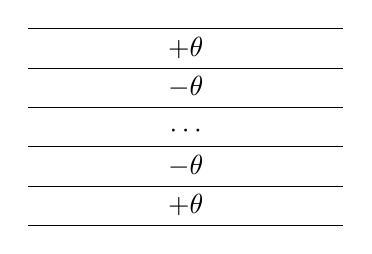
\begin{tikzpicture}
	\draw (0,0) -- (4,0);
	\draw (0,-0.5) -- (4,-0.5) node[midway, above] {$\mathit{+}\theta$};
	\draw (0,-1) -- (4,-1) node[midway, above] {$\mathit{-}\theta$} ;
	\draw (0,-1.5) -- (4,-1.5) node[midway, above] {$\cdots$};
	\draw (0,-2) -- (4,-2) node[midway, above] {$\mathit{-}\theta$};
	\draw (0,-2.5) -- (4,-2.5) node[midway, above] {$\mathit{+}\theta$};
\end{tikzpicture}
\caption{Model for Angle ply laminate}
\end{figure}

\subsection{Stress and Strain in a Lamina}
For a single lamina has a small thickness under plane stress, and it's upper and lower surfaces of the lamina are
free from external loads. According to the Hooke's Law, the three-dimensional stress-strain equations can be reduced to
two-dimensional stress-strain equations. The stress-strain relation in local axis 1-2 is:
\begin{equation}
    \begin{bmatrix}
        \sigma _1\\
        \sigma _2\\
        \tau_{12}
    \end{bmatrix}
    =
    \begin{bmatrix}
        Q_{11} & Q_{12} & 0\\
        Q_{12} & Q_{22} & 0\\
        0      &  0     & Q_{66}
    \end{bmatrix}
    \begin{bmatrix}
        \varepsilon_1\\
        \varepsilon_2\\\gamma_{12}
    \end{bmatrix}
\end{equation}
where $Q_{ij} $are the stiffnesses of the lamina that are related

to engineering elastic constants given by
\begin{equation}
    \begin{split}
    &Q_{11}=\frac{E_1}{1-v_{12}v_{21}}\\
    &Q_{22}=\frac{E_2}{1-v_{12}v_{21}}\\
    &Q_{66}=G_{12}\\
    &Q_{12}=\frac{v_{21}E_2}{1-v_{12}v_{21}}\\
    \end{split}
\end{equation}

where $E_1, E_2, v_{12}, G_{12} $ are four independent engineering elastic constants, which are defined as follows: $E_1 $ is the longitudinal Young's modulus, $E_2 $ is the transverse Young's modulus, $v_{12} $ is the major Poisson's ratio, and $G_{12} $ is the in-plane shear modulus.

Stress strain relation in the global x-y axis:
\begin{equation}\left[\begin{array}{l}\sigma _{x} \\ \sigma _{y} \\ \tau_{xy}\end{array}\right]=\left[\begin{array}{lll}\bar{Q}_{11} & \bar{Q}_{12} & \bar{Q}_{16}\\ \bar{Q}_{12} & \bar{Q}_{22} & \bar{Q}_{26} \\ \bar{Q}_{16} & \bar{Q}_{26} &\bar{Q}_{66}\end{array}\right]\left[\begin{array}{l}\varepsilon_{x} \\ \varepsilon_{y}\\ \gamma_{x y}\end{array}\right]
\end{equation}
where

\begin{equation}
	\begin{array}{l}
		\resizebox{.35\textwidth}{!}{$\bar{Q}_{11}=Q_{11} cos^{4}\theta+Q_{22} sin^{4}\theta+2\left(Q_{12}+2
		Q_{66}\right) sin^{2}\theta cos^{2}\theta$} \\

		\resizebox{.35\textwidth}{!}{$\bar{Q}_{12}=\left(Q_{11}+Q_{22}-4 Q_{66}\right) sin^{2}\theta
		cos^{2}\theta+Q_{12}\left(cos^{4}\theta+sin^{2}\theta \right)$} \\

		\resizebox{.35\textwidth}{!}{$\bar{Q}_{22}=Q_{11} sin^{4}\theta+Q_{22} cos^{4}\theta+2\left(Q_{12}+2
		Q_{66}\right) sin^{2}\theta cos^{2}\theta$} \\

		\resizebox{.4\textwidth}{!}{$\bar{Q}_{16}=\left(Q_{11}-Q_{12}-2
		Q_{66}\right) cos^{3}\theta sin\theta-\left(Q_{22}-Q_{12}-2Q_{66}\right)
	sin^{3}\theta cos\theta$} \\ 
		\resizebox{.4\textwidth}{!}{$\bar{Q}_{26}=\left(Q_{11}-Q_{12}-2
		Q_{66}\right) cos\theta sin^{3}\theta-\left(Q_{22}-Q_{12}-2
Q_{66}\right)cos^{3}\theta sin\theta$}
		 \\ 
	\resizebox{.4\textwidth}{!}	{$\bar{Q}_{66}=\left(Q_{11}+Q_{22}-2 Q_{12}-2 Q_{66}\right)
	sin\theta^{2}cos\theta^{2}+Q_{66}\left(sin\theta^{4}+cos\theta^{4}\right)$}\\
	\end{array}
\end{equation}



The local and global stresses in an angle lamina are related

to each other through the angle of the lamina $\theta $
\begin{equation}\left[\begin{array}{l}\sigma _{1} \\ \sigma _{2} \\ \tau_{12}\end{array}\right]=[T]\left[\begin{array}{l}\sigma _{x} \\ \sigma _{y} \\\tau_{xy}\end{array}\right]
\end{equation}

where
\begin{equation}
	[T]=\left[\begin{array}{ccc}cos^{2}\theta & sin^{2}\theta & 2
		sin\theta cos\theta \\ 
sin^{2}\theta & cos^{2}\theta & -2 sin\theta cos\theta \\
-sin\theta cos\theta
			  & sin\theta cos\theta  &cos^{2}\theta -sin^{2}\theta
\end{array}\right] 
\end{equation}



\subsection{Stress and Strain in a Laminate}
For forces and moment resultants acting on laminates, such as in plate and shell
structures, the relationship between applied forces and moment and displacement
can be given by

\begin{equation} \label{eq:force_and_moments}
	\begin{array}{l}
		\begin{aligned}
	\begin{bmatrix}
		N_x \\
		N_y \\
		N_{xy}
	\end{bmatrix}
	&=
	\begin{bmatrix}
		A_{11} & A_{12} & A_{16} \\
		A_{12} & A_{22} & A_{26} \\
		A_{16} & A_{26} & A_{66} 
	\end{bmatrix}
    \begin{bmatrix}
		\varepsilon_x^0 \\
        \varepsilon_y^0 \\
		\gamma_{xy}^0
    \end{bmatrix}   \\
	&+               
	\begin{bmatrix}
		B_{11} & B_{12} & B_{16} \\
		B_{11} & B_{12} & B_{16} \\
		B_{16} & B_{26} & B_{66} 
	\end{bmatrix}
	\begin{bmatrix}
		k_x \\
		k_y \\
		k_{xy} 
	\end{bmatrix}  \\
\end{aligned} \\ \\
\begin{aligned}
	\begin{bmatrix}
		M_x \\
		M_y \\
		M_{xy}
	\end{bmatrix}
	&=
	\begin{bmatrix}
		B_{11} & B_{12} & B_{16} \\
		B_{12} & B_{22} & B_{26} \\
		B_{16} & B_{26} & B_{66} 
	\end{bmatrix}
    \begin{bmatrix}
		\varepsilon_x^0 \\
        \varepsilon_y^0 \\
		\gamma_{xy}^0
    \end{bmatrix} \\ 
	&+  
	\begin{bmatrix}
		D_{11} & D_{12} & D_{16} \\
		D_{11} & D_{12} & D_{16} \\
		D_{16} & D_{26} & D_{66} 
	\end{bmatrix}
	\begin{bmatrix}
		k_x \\
		k_y \\
		k_{xy} 
	\end{bmatrix}
\end{aligned}
	\end{array}
\end{equation}


$N_x,N_y $  - normal force per unit length

$N_{xy} $  - shear force per unit length

$M_x, M_y $ - bending moment per unit length

$M_{xy} $  - twisting moments per unit length

$\varepsilon^{0}, k $- mid plane strains and curvature of a laminate in x-y coordinates

The mid plane strain and curvature is given by
\begin{equation}
    \begin{split}
    &A_{ij}=\sum_{k=1}^{n}(\overline{Q_{ij}})_k(h_k-h_{k-1})  i=1,2,6, j=1,2,6\\
    &B_{ij}=\frac{1}{2}\sum_{k=1}^{n}(\overline{Q_{ij}})_k(h_k^2 - h_{k-1}^2)  i=1,2,6, j=1,2,6\\
    &D_{ij}=\frac{1}{3}\sum_{k=1}^{n}(\overline{Q_{ij}})_k(h_k^3 - h_{k-1}^3) i=1,2,6, j=1,2,6\\
    \end{split}
\end{equation}

The [A], [B], and [D] matrices are called the extensional, coupling, and bending stiffness matrices,
respectively. The extensional stiffness matrix $[A]$ relates the resultant in-plane forces to the
in-plain strains, and the bending stiffness matrix $[D]$ couples the resultant bending moments to
the plane curvatures.  The coupling stiffness matrix $[B]$ relates the force and moment terms to the
midplain strains and midplane curvatures.

%\section{Failure criteria for a lamina}

Failure criteria for composite materials are more difficult to predict due to
structural and material complexity in comparison to isotropic materials. The
failure process of a composite materials can be regarded from microscopic and
macroscopic points of view. Most popular criteria about the failure of an angle
lamina are in terms of macroscopic failure criteria, which are based on the
tensile, compressive and shear strengths. According to the failure surfaces,
these criteria
\cite{massard1984computer,reddy1987first,fang1993design,soeiro1994multilevel,pelletier2006multi,jadhav2007parametric,omkar2008artificial,choudhury2019failure},
can be classified into two classes: one is called independent failure mode
criteria which includes the maximum stress failure
theory\cite{watkins1987multicriteria}, maximum strain failure theory because
their failure envelop are rectangle; another is called quadratic polynomial
which includes Tsai-Wu\cite{martin1987optimum,soares1995discrete}, Chamis,
Hoffman and Hill criteria because their failure surfaces are of ellipsoidal
shape. In the present study, two most reliable failure criteria is taken,
Maximum stress and Tsai-wu.  Both of these two failure criteria are based on
the stresses in the local axes instead of principal normal stresses and maximum
shear stresses, and four normal strength parameters and one shear stress for a
unidirectional lamina are involved. The five strength parameters are

$(\sigma _1^{T})_{ult}= $ ultimate longitudinal tensile strength(in direction 1),

$(\sigma _1^{C})_{ult}= $ ultimate longitudinal compressive strength,

$(\sigma _2^{T})_{ult}= $ ultimate transverse tensile strength,

$(\sigma _2^{C})_{ult}= $ ultimate transverse compressive strength, and

$(\tau_{12})_{ult}= $ and ultimate in-plane shear strength.

\input{fig/angle_ply_laminate.tex}

\subsection{Maximum stress failure criterion}(MS)


Maximum stress failure theory consists of maximum normal stress theory proposed by Rankine and maximum 
shearing stress theory by Tresca. The stresses applied on a lamina can be resolved into the normal and shear stresses 
in the local axes. If any of the normal or shear stresses in the local axes of a lamina is equal or exceeds the corresponding 
ultimate strengths of the unidirectional lamina, the lamina is considered to be failed. That is,

$\sigma_1 \geq (\sigma _1^{T})_{ult} $ or $\sigma_1 \leq -(\sigma _1^{C})_{ult} $

$\sigma_2 \geq (\sigma _2^{T})_{ult} $ or $\sigma_2 \leq -(\sigma _2^{C})_{ult} $

$\tau_{12} \geq (\tau_{12})_{ult} $  or $\tau_{12} \leq -(\tau_{12})_{ult} $

where $\sigma_1$ and $\sigma_2$ are the normal stresses in the local axes 1 and 2, respectively;
$\tau_{12}$ is the shear stress in the symmetry plane 1-2.

\subsection{Tsai-wu failure criterion}
The TW criterion is one of the most reliable static failure criteria which is derived from the von
Mises yield criterion.  
A lamina is considered to fail
if \begin{equation} \label{eq:tsai_wu}
\begin{split}
	H_1 \sigma_1  & + H_2 \sigma_2 + H_6 \tau_{12} + H_{11}\sigma_1^2 + H_{22} \sigma_2^2 \\
				  & + H_{66}  \tau_{12}^2 + 2H_{12}\sigma_1\sigma_2 < 1
\end{split}
\end{equation}

is violated, where

\begin{equation}
	\begin{split}
		H_{1}&=\frac{1}{\left(\sigma_{1}^{T}\right)_{u l t}}-\frac{1}{\left(\sigma_{1}^{C}\right)_{u l t}} \\
		H_{11}&=\frac{1}{\left(\sigma_{1}^{T}\right)_{u l t}\left(\sigma_{1}^{C}\right)_{u l t}} \\
		H_{2}&=\frac{1}{\left(\sigma_{2}^{T}\right)_{u l t}}-\frac{1}{\left(\sigma_{2}^{C}\right)_{u l t}} \\
		H_{22}&=\frac{1}{\left(\sigma_{2}^{T}\right)_{u l t}\left(\sigma_{2}^{C}\right)_{u l t}} \\
		H_{66}&=\frac{1}{\left(\tau_{12}\right)_{u l t}^{2}} \\
		H_{12}&=-\frac{1}{2} \sqrt{\frac{1}{\left(\sigma_{1}^{T}\right)_{u l
		t}\left(\sigma_{1}^{C}\right)_{u l t}\left(\sigma_{2}^{T}\right)_{u l
		t}\left(\sigma_{2}^{C}\right)_{u l t}}}
	\end{split}
\end{equation}

$H_i$ is the strength tensors of the second order; $H_{ij}$ is the strength
tensors of the fourth order. $\sigma_1$ is the applied normal stress in 
direction 1; $\sigma_2$ is the applied normal stress in the direction 2; and
$\tau_{12}$ is the applied in-plane shear stress.





\begin{figure}
\centering
\begin{tikzpicture}
	\begin{scope}
		%\draw[style=help lines] (-3,-3) grid (3,3);
		\draw (0,0) rectangle (2,3);
		\draw[->] (1.3,1.2) -- (2.6,1.2);
		\draw[->] (1.3,1.2) -- (1.3,3.4);
		\node at (2.2,1) {$X_T$};
		\node at (1.5, 3.2) {$Y_T$};
		\node at (-0.2, 0.9) {$X_C$};
		\node at (1.8, -0.2) {$Y_C$};
	\end{scope}
	\begin{scope}[xshift=6cm,yshift=1.15cm]
		%\draw[style=help lines] (-3,-3) grid (3,3);
		\draw[rotate=30] (0,0) ellipse (2cm and 1cm);
		\draw[->] (0.2,0) -- (0.2,2.2);
		\draw[->] (0.2,0) -- (1.9,0);
		\node at (1.6,-0.2) {$X_T$};
		\node at (0.3, 1.3) {$Y_T$};
		\node at (-1.6, 0) {$X_C$};
		\node at (-0.5, -1.5) {$Y_C$};
	\end{scope}
\end{tikzpicture}
\caption{Schematic failure surfaces for maximum stress and quadratic failure
criteria}
\end{figure}


\subsection{Failure Theories for a Laminate}
If keep increasing the loading applied to a laminate, the laminate will fails. The failure process
of a laminate is more complicate than a lamina, because a laminate consists of multiple plies, and
the fiber orientation, material, thickness of each ply maybe different from the others. In most
situations, some layer fails first and the remains continue to take more loads until all the plies
fail.  If one ply fails, it means this lamina does not contribute to the load carrying capacity of
the laminate. The procedure for finding the first failure ply given follows the fully discounted
method:

\begin{enumerate}
\item Compute the reduced stiffness matrix [Q] referred to as the local axis for each ply using its
	four engineering elastic constants $E_1 $, $E_2 $, $E_{12} $, and $G_{12} $.

\item Calculate the transformed reduced stiffness $[\bar{Q}] $ referring to the global coordinate
	system (x, y) using the reduced stiffness matrix [Q] obtained in step 1 and the ply angle for
	each layer.

\item  Given the thickness and location of each layer, the three laminate stiffness matrices [A],
	[B], and [D] are determined.

\item  Apply the forces and moments, $[N]_{xy}, [M]_{xy} $ solve Equation
	\ref{eq:force_and_moments}, and calculate the middle plane strain $[\sigma ^{0}]_{xy} $ and
	curvature $[k]_{xy} $.

\item Determine the local strain and stress of each layer under the applied load.

\item  Use the ply-by-ply stresses and strains in the Tsai-wu failure theory to find the strength
	ratio, and the layer with smallest strenght ratio is the first failed ply. 
\end{enumerate}

\subsection{Safety factor}
The safety factor, or yield stress, is how much extra load beyond is intended a
composite laminate will actually take. The safey factor is defined as 

\begin{equation} \label{eq:sr}S R=\frac{\text {Maximum Load Which Can Be Applied}}{\text {Load Applied}}
\end{equation}.

%\subsection{Safety factor}
The safety factor, or yield stress, is how much extra load beyond is intended a
composite laminate will actually take, which is an indication of the material's
load carrying capacity. If the value is less then 1.0, it means failure. The safey factor is defined as 

\begin{equation} \label{eq:sr}SF=\frac{\text {Maximum Load Which Can Be
	Applied}}{\text {Load Applied}} {\textstyle .}
\end{equation}

The safety factor based on maximum stress theory is calculated by the following
method: first, the principal stresses($\sigma_1^k$,$\sigma_2^k$, and
$\tau_{12}^k$) are obtained by experiment; evaluate the safety factor along each
direction according to equation \ref{eq:sr}; The minimum value among these
safety factors are denoted as the safety factor of the lamina, $SF_{MS}^k$, it
can be written as 

\begin{align}
	SF_{MS}^k = \text{min of}
	\begin{cases}
		SF_X^k = 
		\begin{cases}
			\frac{X_t}{\sigma_{11}}, \text{ if } \sigma_{11}>0 \\
			\frac{X_c}{\sigma_{11}}, \text{ if } \sigma_{11}<0 \\
		\end{cases} \\
		SF_Y^k = 
		\begin{cases}
			\frac{Y_t}{\sigma_{22}}, \text{ if } \sigma_{22}>0 \\
			\frac{Y_c}{\sigma_{22}}, \text{ if } \sigma_{22}<0 \\
		\end{cases} \\
		SF_S^k =
		\begin{cases}
			\frac{S}{|\tau_{12}|} \\
		\end{cases} \\
	\end{cases} \textstyle{.}
\end{align}


Assuming the composite laminate under a in-plane loading f, the corresponding
stress on local stress in direction 1, local stress in direction 2, and shear
stress for the kth lamina are $\sigma_1 SF_{TW}^k$, $\sigma_2SF_{TW}^k$, and $\tau_{12}SF_{TW}^k$,
respectively. Substitute them into the equation \ref{eq:tsai_wu}, the expression
are given by

$a(SF_{TW}^k)^2 + b(SF_{TW}^k) - 1 = 0 \textstyle{,}$

where 


$a = H_{11}(\sigma_1)^2 + H_{22}(\sigma_2)^2 +H_{66}(\tau_{12})^2 +
2H_{12}\sigma_1 \sigma_2 \textstyle{,} $


$b = H_1\sigma_1 + H_2 \sigma_2 + H_6 \tau_{12} \textstyle{.}$ 


Solve the above equation, the safety factor for the kth lamina is 

$SF_{TW}^k = |\frac{-b+ \sqrt{b^2 + 4a}}{2a}|$.

Then, the minimum of $SF_{TW}^k$ is taken as the safety factor of the
laminate which is written as

$SF_{TW}= \text{ min of } SF_{TW}^k \text{ for } k=1,2,\cdots, m-1,m$ .




\begin{figure}
\setlength{\fboxsep}{0pt}%
\setlength{\fboxrule}{0pt}%
\begin{center}
\resizebox{.95\linewidth}{!}{
		\begin{tikzpicture}
		\tikzstyle{rec} = [rectangle, minimum width=0.8cm,minimum height=0.6cm, text
		centered, draw=black]
			\node (gene11) [rec] {+7};
			\node (gene2) [rec] at ($(gene11.east)+(0.4cm,0)$)  {+7};
			\node (gene3) [rec] at ($(gene2.east)+(0.4cm,0)$)  {+7};
			\node (gene4) [rec] at ($(gene3.east)+(0.4cm,0)$)  {+7};
			\node (gene5) [rec] at ($(gene4.east)+(0.4cm,0)$)  {+7};
			\node (gene6) [rec] at ($(gene5.east)+(0.4cm,0)$)  {+7};
			\node (gene7) [rec] at ($(gene6.east)+(0.4cm,0)$)  {+7};
			\node (gene8) [rec] at ($(gene7.east)+(0.4cm,0)$)  {+7};
			\node (gene9) [rec] at ($(gene8.east)+(0.4cm,0)$)  {-9};
			\node (last) [rec] at ($(gene9.east)+(0.4cm,0)$)  {-9};
			\node[text width=1cm] at ($(gene11.west)+(-0.3cm,0)$) {$P_1$:};
			\node (gene1) [rec] at ($(gene11.east)+(-0.4cm,-0.8cm)$) {+19};
			\node (gene2) [rec] at ($(gene1.east)+(0.4cm,0)$)  {+19};
			\node (gene3) [rec] at ($(gene2.east)+(0.4cm,0)$)  {+19};
			\node (gene4) [rec] at ($(gene3.east)+(0.4cm,0)$)  {+19};
			\node (gene5) [rec] at ($(gene4.east)+(0.4cm,0)$)  {-36};
			\node (gene6) [rec] at ($(gene5.east)+(0.4cm,0)$)  {-36};
			\node (gene7) [rec] at ($(gene6.east)+(0.4cm,0)$)  {-36};
			\node (gene8) [rec] at ($(gene7.east)+(0.4cm,0)$)  {-36};
			\node (gene9) [rec] at ($(gene8.east)+(0.4cm,0)$)  {-36};
			\node (gene10) [rec] at ($(gene9.east)+(0.4cm,0)$)  {-36};
			\node[text width=1cm] at ($(gene1.west)+(-0.3cm,0)$) {$P_2$:};
			\draw[-,white] ($(gene10.north)$)-- ++(0,-1.5cm);
			\node (label1) at ($(gene5.south)+(0cm,-0.5cm)$) {(a): Parents $P_1$ and $P_2$};
		\end{tikzpicture}
}

% offspring
\resizebox{.95\linewidth}{!}{
		\begin{tikzpicture}
			\tikzstyle{rec} = [rectangle, minimum width=0.8cm,minimum height=0.6cm, text
			centered, draw=black]
			\node (gene11) [rec] {+13};
			\node (gene2) [rec] at ($(gene11.east)+(0.4cm,0)$)  {+13};
			\node (gene3) [rec] at ($(gene2.east)+(0.4cm,0)$)  {+13};
			\node (gene4) [rec] at ($(gene3.east)+(0.4cm,0)$)  {+13};
			\node (gene5) [rec] at ($(gene4.east)+(0.4cm,0)$)  {+13};
			\node (gene6) [rec] at ($(gene5.east)+(0.4cm,0)$)  {+13};
			\node (gene7) [rec] at ($(gene6.east)+(0.4cm,0)$)  {-27};
			\node (gene8) [rec] at ($(gene7.east)+(0.4cm,0)$)  {-27};
			\node (gene9) [rec] at ($(gene8.east)+(0.4cm,0)$)  {-27};
			\node (last) [rec] at ($(gene9.east)+(0.4cm,0)$)  {-27};
			\node[text width=1cm] at ($(gene11.west)+(-0.3cm,0)$) {$O_1$:};
			\node (gene1) [rec] at ($(gene11.east)+(-0.4cm,-0.8cm)$) {+22};
			\node (gene2) [rec] at ($(gene1.east)+(0.4cm,0)$)  {+22};
			\node (gene3) [rec] at ($(gene2.east)+(0.4cm,0)$)  {+22};
			\node (gene4) [rec] at ($(gene3.east)+(0.4cm,0)$)  {+22};
			\node (gene5) [rec] at ($(gene4.east)+(0.4cm,0)$)  {+22};
			\node (gene6) [rec] at ($(gene5.east)+(0.4cm,0)$)  {+22};
			\node (gene7) [rec] at ($(gene6.east)+(0.4cm,0)$)  {+22};
			\node (gene8) [rec] at ($(gene7.east)+(0.4cm,0)$)  {+5};
			\node (gene9) [rec] at ($(gene8.east)+(0.4cm,0)$)  {+5};
			\node (gene10) [rec] at ($(gene9.east)+(0.4cm,0)$)  {+5};
			\node[text width=1cm] at ($(gene1.west)+(-0.3cm,0)$) {$O_2$:};
			\draw[-,white] ($(gene10.north)$)-- ++(0,-1.5cm);
			\node (label1) at ($(gene5.south)+(0cm,-0.5cm)$) {(b): Offspring $O_1$ and $O_2$};
		\end{tikzpicture}
}

%mutation
\resizebox{.95\linewidth}{!}{
	\begin{tikzpicture}
	\tikzstyle{rec} = [rectangle, minimum width=0.8cm,minimum height=0.6cm, text
	centered, draw=black]
		\tikzstyle{rec} = [rectangle, minimum width=0.8cm,minimum height=0.6cm, text
		centered, draw=black]
		%\draw[help lines](-3,-3) grid (4,4);
		\node (gene11) [rec] {+13};
		\node (gene2) [rec] at ($(gene11.east)+(0.4cm,0)$)  {+13};
		\node (gene3) [rec] at ($(gene2.east)+(0.4cm,0)$)  {+13};
		\node (gene4) [rec] at ($(gene3.east)+(0.4cm,0)$)  {$\cdots$};
		\node (gene5) [rec] at ($(gene4.east)+(0.4cm,0)$)  {+13};
		\node (gene6) [rec] at ($(gene5.east)+(0.4cm,0)$)  {+13};
		\node (gene7) [rec] at ($(gene6.east)+(0.4cm,0)$)  {-27};
		\node (gene8) [rec] at ($(gene7.east)+(0.4cm,0)$)  {$\cdots$};
		\node (gene9) [rec] at ($(gene8.east)+(0.4cm,0)$)  {-27};
		\node (last) [rec] at ($(gene9.east)+(0.4cm,0)$)  {-27};
		\draw[<->,thick] (gene11.south) .. controls +(1.8,-0.4) .. (gene6.south)
			node[pos=0.5] {11} ;
		\draw[<->,thick] (gene7.south) .. controls +(1.3,-0.4) .. (last.south)
			node[pos=0.5] {7};
		\node[text width=1cm] at ($(gene11.west)+(-0.3cm,0)$) {$O_1$:};

		\node (label1) at ($(gene5.south)+(0cm,-0.8cm)$) {(c): Offspring $O_1$ after
			lenght mutation};

		\node (gene1) [rec] at ($(gene11.east)+(-0.4cm,-1.8cm)$) {+12};
		\node (gene2) [rec] at ($(gene1.east)+(0.4cm,0)$)  {+12};
		\node (gene3) [rec] at ($(gene2.east)+(0.4cm,0)$)  {+12};
		\node (gene4) [rec] at ($(gene3.east)+(0.4cm,0)$)  {$\cdots$};
		\node (gene5) [rec] at ($(gene4.east)+(0.4cm,0)$)  {+12};
		\node (gene6) [rec] at ($(gene5.east)+(0.4cm,0)$)  {+12};
		\node (gene7) [rec] at ($(gene6.east)+(0.4cm,0)$)  {-26};
		\node (gene8) [rec] at ($(gene7.east)+(0.4cm,0)$)  {$\cdots$};
		\node (gene9) [rec] at ($(gene8.east)+(0.4cm,0)$)  {-26};
		\node (last) [rec] at ($(gene9.east)+(0.4cm,0)$)  {-26};
		\node[text width=1cm] at ($(gene11.west)+(-0.3cm,0)$) {$O_1$:};
		\draw[-,white] ($(gene10.north)$)-- ++(0,-1.5cm);
		\node (label1) at ($(gene5.south)+(0cm,-0.5cm)$) {(b): Offspring $O_1$ 
			 after angle mutation};
	\end{tikzpicture}
}
\end{center}
\caption{GA Operators\label{GA:operator}}
\end{figure}

\section{Methodology}
\subsection{Objective function}
The optimization problem can be formulated by searching the optimal stacking
sequence of composite laminate.  There are two design variables here, the angles
in the laminate, and the number of layers that each fiber orientation has. The
objective function is formulated as

\begin{equation}
	\begin{split}
    	F  &= 2t_0 \sum_{k=1}^n n_k  \textstyle{,}\\
    	   &SF_{MS} \geq 1 \textstyle{,} \\
    	   &SF_{TW} \geq 1 \textstyle{.}
	\end{split} 
\end{equation}

The first term represents the total thickness of the composite laminates, $t_0$
is the ply thickness; $n_k$ is the number of plies in the kth lamina, in which
the fiber orientation is $\theta_k$. The constraints here are two safety
factors should not less than 1, which means  $SF_{MS} \geq 1$, and $SF_{TW} \geq
1$, respectively.

\subsection{Encoding}
Due to the simplicity and efficiency of float representation, this encoding
method is implemented to represent a possible solution. As shown in Figure \ref{GA:operator}
 (a), these two chromsomes represent a $[+8_{7}/-9_{2}]_s$
carbon T300/5308 laminated composite, and $[+19_{4}/-36_{6}]_s$, respectively.
Becasue the laminate adopted in this paper is symmetric to its mid-plane, so
only half needs to be encoded.

\subsection{Selection}
The purpose of the selection operator is to choose mating pool to produce
alternative solutions of better fitness. Traditional methods of selecting
strategies only take the fitness of individuals into account, however, due to 
the existence of constraint, various selection schemes are implemented to
select the mating set. Based on different selection schemes, the parents of
next generation can be divided into  three groups: proper groups, active groups,
and potential groups according to different selecting methods. 

Proper parents mean in which individual fullfills the constraints, which are
chosen by the individual's fitness, individuals with better fitness are more
likely to be chosen if they fit the constraint; active group means that
individual within this group is supposed to always exist in the parents during the GA, which
are selected by fitness, ignoring the constraint; The individuals from the active
group may not correspond to feasible solutions, but their existence enriches the
variety of the gene clips.  Potential group means that individuals are likely to turn
into proper individual after a couple of generations, and potential individuals
are chosen by constraint function, the more the individual fulfills the
constraint, the more possibility it will be selected.

\subsection{Crossover}
The crossover operator happens among these three groups. the child of two proper
groups is more likely to be a proper individual which can be used to obtain an
alternative feasible solution. the child of an active individual and a potential
individual can significantly change the gene of an active individual's chromosome,
which makes the individual evolve toward a new direction. The offspring of two
active individuals are more likely to be an active individual, which can maintain
the active group.  The figure.\ref{GA:operator} (b) shows two children $O_1$
and $O_2$ from two parents $P_1$ and $P_2$, each angle $C_a$ and its length 
$C_l$ of a child are obtained by the following formula
\begin{align} 
	\begin{cases}
	C_a &= (P1_a + P2_a)/2 \\
	C_l &= (P1_l + P2_l)/2 
\end{cases} \textstyle{.}
\end{align}
\begin{table}[tb]
\caption{Comparison of the carbon/epoxy, graphite/epoxy, and glass/epoxy properties}
\centering
\begin{adjustbox}{width=0.5\textwidth}
\label{tab:mat}
\begin{tabular}{lccccc}
\toprule
Property								   & Symbol				  & Unit  &  Carbon/Epoxy&  Graphite/Epoxy  &  Glass/Epoxy   \\
\midrule
Longitudinal elastic modulus			   & $E_1$				  & GPa   &  116.6       &  181             &  38.6           \\
Traverse elastic modulus				   & $E_2$				  & GPa   &  7.67        &  10.3            &  8.27           \\
Major Poisson's ratio					   & $v_{12}$			  &       &  0.27        &  0.28            &  0.26           \\
Shear modulus							   & $G_{12}$			  & GPa   &  4.17        &  7.17            &  4.14           \\
Ultimate longitudinal tensile strength     & $(\sigma_1^T)_{ult}$ & MP    &  2062        &  1500            &  1062            \\
Ultimate longitudinal compressive strength & $(\sigma_1^C)_{ult}$ & MP    &  1701        &  1500            &  610             \\
Ultimate transverse tensile strength       & $(\sigma_2^T)_{ult}$ & MPa   &  70          &  40              &  31              \\
Ultimate transverse compressive strength   & $(\sigma_2^C)_{ult}$ & MPa   &  240         &  246             &  118              \\
Ultimate in-plane shear strength           & $(\tau_{12})_{ult}$  & MPa   &  105         &  68              &  72               \\
Density                                    & $\rho$               & $g/cm^3$ &  1.605    &  1.590           &  1.903               \\
Cost                                       &                      &       &  8           &  2.5             &  1               \\
\bottomrule
\end{tabular}
\end{adjustbox}
\end{table}

\subsection{Mutation}
A mutation direction is imposed on the mutation operator which to make sure the
individual evolving toward the right direction. The mutation direction, denoted
by $md$, is an n dimensional vector corresponding to the number of constraints, it
is decided by the constraint thresholds $CT_i$ and the current individual's
constraint value, denoted as $CV_i$,  The mutation vector can be obtained by the
following formula

\resizebox{.9\linewidth}{!}{
	$\text{md} = [CT_1, \cdots, CT_{n-1}, CT_n] -  [CV_0, \cdots, CV_{n-1}, CV_n] \textstyle{.}$

}

During this operator, the mutation procedure is consist of two phases: the length
mutation of the chromosome, and the angle mutation of the chromosome.  Because the
chromosome's length is positively correlated with the individual's fitness, the
coefficient of length mutation denoted by $C_l$, if $\sum_{i=1}^{N}{CT_i}$ great
than $\sum_{i=1}^{N}{CV_i}$ , the mutation length is restricted to the range
$[0,(C_l \sum_{i=1}^{N}{(CT_i-CV_i)})/N]$, which means increase the chromosome's
length; Assuming a $[+13_6/-27_4]_s$ T300/5308 carbon/epoxy composite
laminate under the loading $N_{x} = N_{y} = 10$ MPa m, it's property as shown
in table \ref{tab:T300/5308}. According to CLT and
failure theory, the two safety factors $SF_{MS}$ and $SF_{TW}$ are  0.0539, and
0.0540, respectively. So the mutation vector and is $[0.9461,0.9460]$, assuming
the length mutation coefficient is 20, so the mutation range is from 0 to 18. A
random number is generated from the range $[0, 18]$, supposing the outcome is
13, then a length generator is used to a list, the its sum is 13, suppose the
list is [5, 8], the laminate after mutation is $[13_{11}/-27_{12}]_s$.

If the $\sum_{i=1}^{N}{CT_i}$ less than $\sum_{i=1}^{N}{CV_i}$, the
mutation length is restricted to the range $([\sum_{i=1}^{N}{CT_i-CV_i})/N,0]$,
which means the individual's fitness exceeds the threshold value, and decrease
the chromsome's length.  Assuming a $[+33_{35}/-29_{26}]_s$ T300/5308 laminate
is under loading $N_{x}=10$ MPa, and $N_{y}=5$ MPa, then, it's $SF_{MS}$
constraint and $SF_{TW}$ values are  1.0912, 1.0747, respectively.
because the length mutation is 20, so the mutation range is from -2 to 0. This
would decrease the chromosome's length. 
\begin{align}
	\text{LM} = 
	\begin{cases}
		\resizebox{.35\textwidth}{!}{$[0,(C_l \sum_{i=1}^{N}{(CT_i-CV_i)})/N], \text{ if }  \sum_{i=1}^{N}{CT_i} > 
		\sum_{i=1}^{N}{CV_i}$}\\
		\resizebox{.35\textwidth}{!}{$[(C_l \sum_{i=1}^{N}{(CT_i-CV_i)})/N,0], \text{ if }  \sum_{i=1}^{N}{CT_i} < 
		\sum_{i=1}^{N}{CV_i}$}\\
	\end{cases} 
\end{align}

The relationship between the angles in the composite laminate and the
chromosome's fitness is unclear, so the mutation direction of chromosome's angle
is random. The coefficient angle mutation is $C_a$, the angle mutation range is
$[0,C_a \sum_{i=1}^{N}{(|CT_i-CV_i|)}]$ or $[C_a
\sum_{i=1}^{N}{(-|CT_i-CV_i|)},0]$. It is can be written as

\begin{align}
	\text{P(AM)} =  
	\begin{cases}
		0.5, \text{ AM = }[0,C_a \sum_{i=1}^{N}{(|CT_i-CV_i|)}] \\ 
	    0.5, \text{ AM = }[C_a \sum_{i=1}^{N}{(-|CT_i-CV_i|)},0]
	\end{cases} \textstyle{.}
\end{align}

\section{Result and Discussion}
We have conducted experiment by the use of the generated data set. This data
set is randomly partitoned into a training set and a test.

Figure \ref{fig:train-process} shows five ANNs with different topologies, quite
different results have been observed when different architectures are adopted.
It is clear that architecture whose mean of average difference is less than the
rest.


\begin{figure}
	\centering
	\def\svgwidth{\columnwidth}
	\import{fig/}{pre_train.pdf_tex}
	\label{fig:train-process}
\end{figure}

Table \ref{tab:simu} shows part of the valudation.
\begin{table}[!tb]
	\centering
	\caption{ANN predictions of the Tsai-wu and MS strength ratio with the
	numberical results obtained by CLT.}
	\label{tab:simu}
	\begin{adjustbox}{width=0.5\textwidth}
	\begin{tabular}{cccc|cc|cc}
		\toprule
		\multicolumn{4}{c}{\textbf{Input}} &  \multicolumn{4}{c}{\textbf{Output}} \\
		\midrule
		Load  &  \makecell{Laminate \\ Structure }  & \makecell{Material \\ Property} & \makecell{Failure \\  Property}  &
		\multicolumn{2}{c}{ \makecell {CLT \\MS  Tsai-Wu}} & \multicolumn{2}{c}{ \makecell {ANN \\MS  Tsai-Wu}}\\
		\midrule
		-10,40,20  &  26,-26,168,1.27 & 116.6,7.67,0.27,4.17 & 2062.0,1701.0,70,240,105 & 0.342 & 0.476 & 0.351 & 0.492 \\
		20,-70,-30 &  10,-10,196,1.27 & 181.0,10.3,0.28,7.17 & 1500.0,1500.0,40,246,68  & 0.653 & 0.489 & 0.612 & 0.445 \\ 
		60,-20,0   &  82 -82,128,1.27 & 181.0,10.3,0.28,7.17 & 1500.0,1500.0,40,246,68  & 1.663 & 0.112 & 1.673 & 0.189 \\
		\bottomrule
	\end{tabular}
	\end{adjustbox}
\end{table}



\begin{figure}
	\centering
	\def\svgwidth{\columnwidth}
	\import{fig/}{post_train.pdf_tex}
	\label{fig:final_train}
\end{figure}


Comparing the strength ratio outputs based on CLT and ANN from
Tab.\ref{tab:simu}, we can see that the calculation of strength ratio can be
achieved using a two-layer neural network, without the intensive computation of
matrix multiplication.





\section{Conclusion}
In this paper, an evolutionary artificial neural network model was developed to
predict the strength ratio of laminated composite material under in-plane
loading. We review the use of genetic algorithms and artificial neural networks
as an alternative approach for calculating the strength ratio of an angle ply
laminate under in-plane loading. Traditionally, it is obtained through CLT and
corresponding failure criteria, such as Maximum Stress theory and Tsai-Wu
failure theory.

The main contribution of this work is as follows: 1) propose a two-layer diagram
model for designing a sophisticated neural network in simulating the calculation
of strength ratio, and use a genetic algorithm to explore the search space. 2)
suggest an efficient method to compute the strength ratio instead of adopting
the two-step procedure based on classical lamination theory and related failure
criteria. Compared with experimentally obtained data, it is demonstrated that
ANN is an efficient and simple tool to compute the strength ratio, instead of
the complex analytical mathematical model. Our findings underline the practical
applicability of ANN on the analysis of composite material.

There are more improvements we can make over the search strategy and application
in the area of laminated composite material. The future work is to develop a
more sophisticated ANN, which not only can predict the properties for angle ply
laminate, but also the other type of laminated composite material.


%\section{Acknowledgment}
The paper is based on the work supported by China Scholarship Council with
the code number 201806630112

